\documentclass[a4j,12pt]{jreport}
\makeatletter
\usepackage{url}
\usepackage{jtygm}
\usepackage{ascmac}
\usepackage[dvipdfmx]{graphicx}
\usepackage{amsmath,amssymb}
\usepackage{multicol}
\usepackage{listings}
\usepackage{makeidx}
\usepackage{ccaption}
\usepackage{here}
\usepackage{subfigure}
\usepackage{enumerate}
\usepackage[dvipdfmx]{color}
\usepackage{fancybox}
\usepackage{geometry}
\usepackage{ascmac}
\usepackage{titletoc}
\usepackage{titlesec}
\usepackage{framed}
\usepackage{longtable}
\usepackage{ulem}
\usepackage{anyfontsize}
\usepackage{wrapfig}
\usepackage{bm}

\renewcommand{\lstlistingname}{リスト}

\newcommand{\minisec}[1]{
\subsubsection{【#1】}
}

\geometry{
body={384pt,574pt},
hmargin={2.0cm,2.0cm},
vmargin={2.5cm,2.0cm},
bindingoffset=0.5cm,
twoside
}

% 付録の始まり
\newcommand{\beginappendix}{
  % 章番号の書式変更
  \setcounter{chapter}{0}
  \renewcommand{\prechaptername}{付録}
  \renewcommand{\postchaptername}{} 
  \renewcommand{\thechapter}{\@Alph\c@chapter}
  \renewcommand{\thesection}{\@Alph\c@chapter.\@arabic\c@section}
  \renewcommand{\thesubsection}{\@Alph\c@chapter.\@arabic\c@section.\@arabic\c@subsection}
}

%図番号の書式変更
  \renewcommand{\thefigure}{%
  \thechapter.\arabic{figure}}
  \@addtoreset{figure}{chapter}
\makeatother


\newcommand{\ruby}[2]{%
\leavevmode
\setbox0=\hbox{#1}%
\setbox1=\hbox{\tiny #2}%
\ifdim\wd0>\wd1 \dimen0=\wd0 \else \dimen0=\wd1 \fi
\hbox{%
\kanjiskip=0pt plus 2fil
\xkanjiskip=0pt plus 2fil
\vbox{%
\hbox to \dimen0{%
\tiny \hfil#2\hfil}%
\nointerlineskip
\hbox to \dimen0{\mathstrut\hfil#1\hfil}}}}

\makeatletter
\lstset{% 
language={C}, 
frame=trbl,% 
basicstyle={\small},% 
identifierstyle={\small},% 
commentstyle={\small\ttfamily},% 
keywordstyle={\small\bfseries},% 
ndkeywordstyle={\small},% 
stringstyle={\small\ttfamily}, 
tabsize=2,
breaklines=true, 
frame=none,
columns=[l]{fullflexible},% 
numbers=left,% 
xrightmargin=0zw,% 
xleftmargin=3zw,% 
numberstyle={\scriptsize},% 
stepnumber=1, 
numbersep=1zw,% 
backgroundcolor={\color[gray]{.90}},
} 

%footnoteにおいてverbを有効にする設定
\long\def\@footnotetext{%
  \insert\footins\bgroup
    \normalfont\footnotesize
    \interlinepenalty\interfootnotelinepenalty
    \splittopskip\footnotesep
    \splitmaxdepth \dp\strutbox \floatingpenalty \@MM
    \hsize\columnwidth \@parboxrestore
    \protected@edef\@currentlabel{%
       \csname p@footnote\endcsname\@thefnmark
    }%
    \color@begingroup
      \@makefntext{%
        \rule\z@\footnotesep\ignorespaces}%
      \futurelet\next\fo@t}
\def\fo@t{\ifcat\bgroup\noexpand\next \let\next\f@@t
                                \else \let\next\f@t\fi \next}
\def\fo@t{\bgroup\aftergroup\@foot\let\next}
\def\f@t#1{#1\@foot}
\def\@foot{\@finalstrut\strutbox\color@endgroup\egroup}

\renewcommand{\seename}{→}
\makeatother

%-----目次及び見出し-----
\contentsmargin{0pt}
  \titlecontents{chapter}[5.6pc]
  {\addvspace{10pt}\bfseries}
  {\contentslabel[\thecontentslabel]{4.6pc}}
  {}
  {\hfill\normalfont\thecontentspage}

  \titlecontents{section}[4.8pc]
  {\addvspace{4pt}\bfseries}
  {\contentslabel[\thecontentslabel]{2.8pc}}
  {}
  {\dotfill\thecontentspage}

  \titlecontents{subsection}[6.4pc]
  {\addvspace{2pt} }
  {\contentslabel[\thecontentslabel]{3.4pc}}
  {}
  {\dotfill\normalfont \thecontentspage }

 \titleformat{\chapter}[frame]
  {\small}
  {\filright
   \large
  第 \thechapter 章}
  {8pt}
  {\LARGE\bfseries\filcenter}

\titleformat{\section}[hang]{\large\bfseries}
{\colorbox{black}{\color{white}\thesection}}{12pt}{}%
[{\titlerule[1pt]}]

\titleformat{\subsection}[block]
{\normalfont\bfseries}{\fbox{\itshape\thesubsection}}{1em}{}
[{\titlerule[0.5pt]}]

\titleformat{\subsubsection}
{\normalfont\bfseries}{\itshape\thesubsubsection}{1em}{\doublebox}


 \titlespacing{\chapter}{0pt}{4pt plus 2pt minus 1pt}{2pt plus 2pt minus 2pt}
 \titlespacing{\section}{0pt}{0pt plus 0pt minus 0pt}{0pt plus 0pt minus 0pt}
 \titlespacing{\subsection}{0pt}{0pt plus 0pt minus 0pt}{0pt plus 0pt minus 0pt}
 \titlespacing{\subsubsection}{0pt}{0pt plus 0pt minus 0pt}{0pt plus 0pt minus 0pt}

\newenvironment{code}{
\VerbatimEnvironment
\begin{quote}
\begin{Verbatim}	
}
{
\end{Verbatim}
\end{quote}
}

\newenvironment{problems}
{
  \renewcommand\labelenumi{\doublebox{\arabic{enumi}}}
  \begin{enumerate}
}{
  \end{enumerate}
  \renewcommand\labelenumi{\arabic{enumi}.}
}


\makeindex

\begin{document}
\makeatletter
\renewcommand{\thelstlisting}{\thechapter.\@arabic\c@lstlisting}
\makeatother

\title{{\normalsize 人の言を通す}\\ 通信ひとわたり}
\author{達哉ん}
\date{2018年6月執筆開始}
\maketitle
%\begin{titlepage}
%\vspace{24pt}
%\textbf{\large 理論と実習の両面から学ぶ}
%\begin{center}
%\includegraphics[width=0.95\linewidth,keepaspectratio]{title1.eps}
%\end{center}
%\vspace{120pt}
%\begin{center}
%\includegraphics[width=0.75\linewidth,keepaspectratio]{title2.eps}
%\end{center}
%\vspace{120pt}
%\begin{flushright}
%\textbf{\LARGE 達哉ん 著}
%\end{flushright}
%\end{titlepage}
%\newpage

\setlength{\parskip}{3ex plus 0.8ex minus 0.4ex}

\pagenumbering{roman}
\chapter*{はじめに}
\input{start}

\setlength{\parskip}{1ex plus 0.0ex minus 0.0ex}
\tableofcontents

\newpage

\setlength{\parskip}{3ex plus 0.8ex minus 0.4ex}
\pagenumbering{arabic}
\setcounter{chapter}{-1}
\chapter{「伝える」歴史}
\input{chap00}

\part{情報の記録}

\chapter{デジタルデータの記録}
\input{chap01}

\chapter{アナログデータの記録}
現実世界において対面する多くのデータは離散的ではない。音声や映像は無論のこと、道程や時間も連続的なデータ(アナログデータ)である。アナログデータをそのままに記録・伝達することは多くの場合難しい。そのため、保存にあたっては復元可能なデジタルデータへと置き換えて保存される場合が多い。

本章では、まずアナログデータをそのまま連続的な量として記録できる例を説明する。次いで、デジタルデータへの置き換えについて、その手法と制約、影響等を論ずる。

\section{連続データの記録}

デジタルデータの保存方法がなかった頃、あるいは乏しかった頃、アナログデータは変換なしにそのまま保存されていた。図画はその最も原始的なものであろう。風光明媚な風景を伝えたいと描かれた風景画、その人物の偉大さを讃えた肖像画、建物の設計図などは、人間の視覚による差異や筆致の巧拙を別にすれば、おおよそそのままに伝えている。あるいは立像なども直接保存する一例と言えよう。

時代は下り、人はアナログのデータを直接に、あるいは必要に応じて媒体を変換させつつも連続性を保ったまま保存する術を開発してきた。ここでは、光・音・運動の3例を紹介する。

\subsection{光の保存例:写真}
光をそのまま保存している例としては写真がある。写真はカメラを用いて図\ref{fig2_1}に示すように光をフィルムに投影する。
\begin{figure}[htbp]
\centering
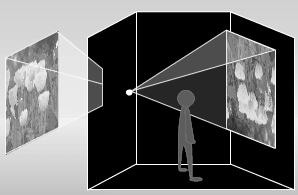
\includegraphics[width=0.6\linewidth,keepaspectratio,bb=0 0 298 195]{fig/fig2_1.png}
\caption{ピンホールカメラ。Canonサイトより引用}\label{fig2_1}
\end{figure}

フィルムには感光体があり、この感光体が受けた光に応じて変化を起こす。記録自体はこれで完了である。実際に読み出すには、この変化した感光体を薬品などに浸して化学変化させて再度発色させるなどの工程が行われる。一般には現像と呼ばれる工程である。

フィルムの化学変化を光によって起こすという方法で、そのままでは消えてしまう光を物質の際によって保存しているのが写真なのである。

\subsection{音の保存例:レコード}
音声・音楽の保存というのは非常に顕著な変化を見せている。戦後の頃には、レコードが主たる媒体であった。レコードは薄い板の両面に音楽のデータを刻む事ができる媒体だった。現代でも稀に"両A面シングル"などという呼び名があるが、これは元々レコードにA面とB面という区別があったことから出来た言葉である。

その後、ABがなくなり、CDへと移った(桂文珍「心中恋電脳」)。コンパクト・ディスクは片面のみにデジタルデータで保存を行い、これを光学的に読み取って音声へと変換することで音楽を鳴らし始めた。ここがアナログとデジタルの分かれ目である。AB…つまりレコードはアナログであったが、CDはデジタルということである。アナログとデジタルの変換をA/D変換などと書くことがあるが、なるほど、A(B)/(C)Dの変換と考えると確かにこの変化は顕著である。…洒落はともかく、このデジタルとなった音楽をインターネットを介して運ぶようになったのが現代のダウンロードによる音楽配信である。ことほど左様に音声・音楽データの保存は記録や通信の変化に対応しているのである。

レコードでの音楽の保存はアナログな音を「そのままに」保存しているのであるが、これは一体どういう原理であろうか。

音声というのは空気の振動である。この空気の振動を保存すれば良い…これがレコードの最も基本的な考えである。空気の振動を適当なもの(通常は針)に集音して伝え、下の面で回転している(記録前の)レコードに当てる。これにより、レコードが振動に合わせて削られる。再生するときは、逆にレコードの削れた面をなぞるように針をあて、この振動を増幅させて音声とする。

空気の振動ということでは動きもするし減衰もする。そのため、空気の振動をそのまま別の振動へと変換して保存するのがレコードという媒体の原理である。

\subsection{運動の保存例:地震計}
レコードは空気の振動であったが、同じ原理を用いて地面の振動=地震の揺れを記録するのが地震計である。

地震計は錘(おもり)に糸をつけた振り子を用意し、錘を不動点として地面の揺れを記録する。(図\ref{fig2_2})
\begin{figure}[htbp]
\centering
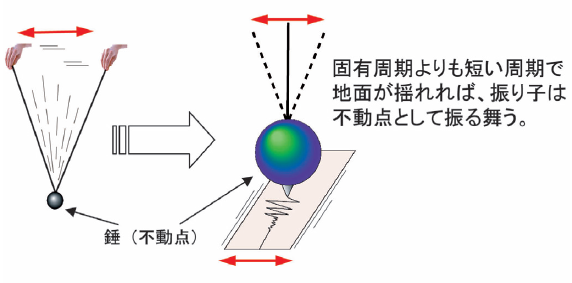
\includegraphics[width=0.6\linewidth,keepaspectratio,bb=0 0 572 283]{fig/fig2_2.png}
\caption{地震計の原理。札幌管区気象台サイトより引用}\label{fig2_2}
\end{figure}

振り子の糸の端を素早く左右に動かした場合、錘は動かない。そのため、錘の下にペンをつけ地面に紙を置くと紙だけが揺れるため地面の動きを記録することができる。これを複数の方向(東西・南北・上下)用意すれば、地震の3次元的な揺れをそのまま記録することができる。レコードと違い、これをそのままに再現するのは困難であるが(また、再現されると非常に迷惑でもあるが)、地震の状況を伝える資料として保存する、あるいは伝えるのには格好の方法と言えよう。


\section{デジタルデータへの変換}

アナログデータの保存の例を示してきたが、アナログデータは必ずしも移行や保存が楽ではなく、また通信の観点から見ても例えば地震計をそのままに伝送するには紙を運送する必要がある。また、レコードのように専用の機器が必要になる場合も多く、取扱が簡便であるとは言い難い。そこで、汎用性を持った記録・通信のためにデジタルデータへ変換して保存するということが考えられる。

アナログデータをデジタルデータに変換する場合というのは、連続性のあるものから代表値を選び出してそれを順に記録することとなる。これは、次の三つの手順からなる。
\begin{enumerate}
\item \textbf{標本化}\index{ひょうほんか@標本化}(Sampling):アナログデータから代表値(サンプリング値・標本値)を取得する。
\item \textbf{量子化}\index{りょうしか@量子化}(Quantization):サンプリング値をデジタルで表現可能な最も近い値へと丸める。
\item \textbf{符号化}\index{ふごうか@符号化}(Encoding):量子化された値(量子化値)を記録できる形式に変換する(多くはビット列となる)。デジタルデータの符号化と同様である。
\end{enumerate}

この途上において、最初に歴史に学んだ通り、取捨選択されている部分が存在する。アナログとデジタルを比較した文脈においては、しばしば「デジタルにはないアナログの良さ」が標榜されているが、その多くはこの標本化や量子化において捨象された部分を指す。捨象された部分というのは伝達に不都合であるとか影響が少ない、あるいはそもそも不必要といった部分であるため、伝達や記録と言った主目的を達するために、本質的でない部分を犠牲にしているというのがデジタルへの変換の基本的な考えである。これはそのまま、「微細な心情等は伝わりづらいが効率的」とされるデジタルデータと、「扱いは面倒だが機微が伝わる」とされるアナログデータの印象にも繋がっていると言えよう。

閑話休題。上記のようにデジタルデータへと変換し保存された後は、保存されたデータを読み取ってその値を適切につなぐことで原データの近似データを得られる。この近似データが十分良い近似であればアナログデータの保存という目的は達せられたと言える。では、この適切な近似データを得るためにはどうすればよいだろうか?以後、変換の各手順とともに良質な変換を担保する条件を見ていこう。

\section{アナログデータの標本化}

アナログデータの標本点を定め、標本値を取得するのがアナログデータの標本化である。つまり、連続的なデータの何点かを取り、その点の値を取得するという動作を標本化と呼ぶ(図\ref{fig2_3})。

\begin{figure}[htbp]
\centering
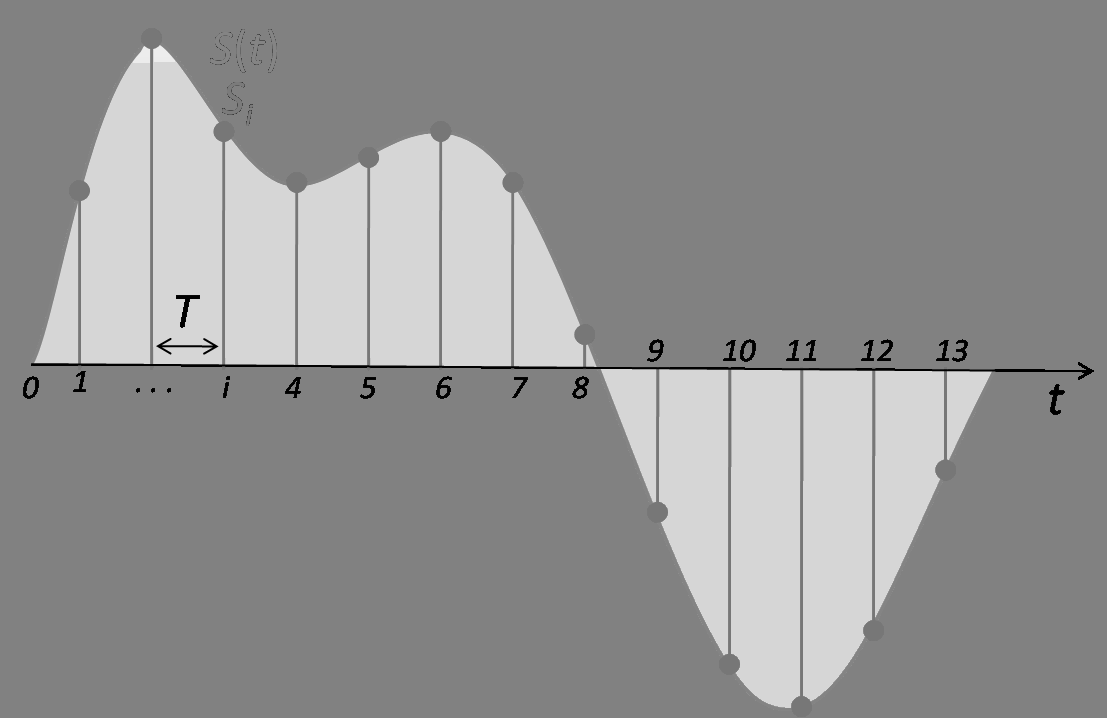
\includegraphics[width=0.6\linewidth,keepaspectratio,bb=0 0 1107 718]{fig/fig2_3.png}
\caption{標本化の例。各点における縦線が標本値を示す。Wikipediaより引用}\label{fig2_3}
\end{figure}

得られた標本値を適切に結ぶことができれば原データを復元できる。しかし、標本値が十分な個数なければ原データを正確に・精確に復元することは困難になるだろう。だからといって過剰に多くの点を取ってしまえばデータの量が嵩んでしまうのは目に見えている。これらの観点からすれば、原データを復元するに必要な最小限のデータを標本値として取得することが望ましい。では、どのようなデータをとれば原データを復元できるだろうか?その答えの源流は、19世紀初頭頃の物理学の話に遡る。

\subsection{Fourierの夢}

18世紀から19世紀にかけて活躍した、フランスの数学者・物理学者Jean Baptiste Joseph Fourier男爵は、ある物体中で熱がどのように伝わるのかを表す熱伝導方程式を導出した。もっとも、熱伝導方程式は方程式と言っても一般にいう代数方程式―未知数を含む関係式があり、限られた値しか認められないような等式―ではなく、関数方程式―未知の関数に関する関係式があり、これを満たす関数が限られる等式―である。つまり「あてはまる数値を求める方程式」ではなく「あてはまる関数を求める方程式」である。

Fourierは著書「熱の解析的理論」において、"任意の関数は、三角関数\footnote{ここでは$\sin,\cos$のこと。}の級数\footnote{無限和のこと。}で表すことができる"と主張した。Fourier自身が与えたこの主張に対する証明は不十分であったが、後世の数学者により「ほとんどあらゆる」関数について三角関数の総和形式で表されることが示された。方程式論や方程式の解法に終生興味を持ち続けたFourierの夢が花開いたといえる。このように、関数を三角関数の総和形式に表すことを、\textbf{Fourier展開}\index{Fourierてんかい@Fourier展開}あるいは\textbf{Fourier変換}\index{Fourierへんかん@Fourier変換}と呼ぶ\footnote{一般には、有限区間での総和をFourier展開、無限区間での総和をFourier変換と呼び分けている。}。

三角関数は周期的に変化する。このため、三角関数は波を表していると言える。波の周期の逆数を\textbf{周波数}\index{しゅうはすう@周波数}と呼ぶ。Fourier展開とは、異なる周波数の波を十分な個数集め、必要な程度に増幅あるいは減衰させて足し合わせることによって関数を表せるという主張である。各々の周波数における増幅あるいは減衰を表す係数を\textbf{周波数スペクトル}\index{しゅうはすうすぺくとる@周波数スペクトル}と呼ぶ。

現実に扱うアナログデータにおいて、Fourier展開が出来ないようなデータはまずない。このため、アナログデータは三角関数の総和形式によって表すことができるといえる。そして、この三角関数の総和形式から、「どのように標本点を取ればよいのか」という答えが導かれる。そう、原データをFourier展開した際に含まれる周波数スペクトルを求めるに必要なだけのデータを取れば良い、ということである。

\subsection{【補遺】Fourier展開の数学的議論}
\begin{center}
\begin{minipage}[]{0.75\linewidth}
\begin{screen}
\begin{center}
本節は大筋に影響せず、やや高度な(大学程度の)数学を扱う。\\
難解あるいは興味索然たるものと感じる折には\\
飛ばして次節を読まれたい。
\end{center}
\end{screen}
\end{minipage}
\end{center}

先に書いたFourier展開について、もう少し数学的に議論しておこう。Fourier展開の主張とは、ある関数$f(x)$について
\begin{equation}
f(x)=\frac{a_0}{2} + \sum^{\infty}_{k=1} \left( a_k \cos f_kx + b_k \sin f_kx \right) \label{eq_2_1}
\end{equation}
が成立するということである。但し、最初の定数項は調整のために係数をつけている。各係数$a_k,b_k$が周波数スペクトルを、$f_k$が周波数を表す。

ここで、$f(x)$の周期が$L$であるとしたとき、これを表すための周波数$f_k$は
\begin{equation}
f_k=\frac{k\pi}{L}
\end{equation}
として表される。このとき、三角関数には直交性がある\footnote{2つの関数同士の積を周期積分したとき、同一の関数でなければ0となり、同一の関数であれば0でない有限値となる}ため、式(\ref{eq_2_1})の両辺に適当な周波数成分をかけて周期積分することにより、次のように係数を求めることができる。
\begin{equation}
a_k=\int^{L}_{-L} f(x) \cos f_kx dx \quad , \quad b_k=\int^{L}_{-L} f(x) \sin f_kx dx \label{eq_2_2}
\end{equation}

アナログデータの再現とは、離散化されたデータを用いて$a_k,b_k$を計算し、元の$f(x)$を得ることである。つまり、アナログデータから変換された後のデジタルデータは$a_k,b_k$を元通り求めるのに必要なデータと言える。なお、この計算は、離散フーリエ変換(discrete Fourier transform,DFT)あるいはそれを高速化した高速フーリエ変換(fast Fourier transform,FFT)と呼ばれる手法による。

\subsection{標本化定理}

Fourierの主張により、原データをFourier展開した際に含まれる周波数スペクトルを求めるに必要なだけのデータをサンプリングすれば良いことまでは前節で見えてきた。では、「必要なデータ」とは一体どういうデータであろうか。それを示すのが\textbf{標本化定理}\index{ひょうほんかていり@標本化定理}あるいは\textbf{サンプリング定理}\index{さんぷりんぐていり@サンプリング定理|see{標本化定理}}である。この定理は、1928年にHarry Nyquistによって予想され、1949年にClaude Elwood Shannonと日本の染谷 勲によってそれぞれ独立に証明された。この予想者あるいは証明者の名前を取り、\textbf{ナイキストの定理}\index{ないきすとのていり@ナイキストの定理|see{標本化定理}}、\textbf{ナイキスト・シャノンの定理}\index{ないきすとしゃのんのていり@ナイキスト・シャノンの定理|see{標本化定理}}、\textbf{染谷・シャノンの定理}\index{そめやしゃのんのていり@染谷・シャノンの定理|see{標本化定理}}(主に日本)と呼ばれることもある。

標本化定理は次のことを主張している。
\begin{itembox}[l]{標本化定理}
原信号に含まれる最大周波数成分の2倍以上の周波数でサンプリングされたデータがあれば原信号を完全に再構成できる。逆にサンプリングデータの周波数が原信号の2倍を下回る場合は完全に再構成できるとは限らない。
\end{itembox}

この定理において、原信号に含まれる周波数の2倍という値が出てくるが、この周波数を\textbf{ナイキスト周波数}\index{ないきすとしゅうはすう@ナイキスト周波数}と呼ぶ。また、サンプリングの周波数(=サンプリング間隔の逆数)を\textbf{サンプリング周波数}\index{さんぷりんぐしゅうはすう@サンプリング周波数}と呼ぶ。この言葉を用いて換言すれば、標本化定理とは「原信号の完全復元にはナイキスト周波数以上のサンプリング周波数でサンプリングされたデータが必要である」と言える。

原データの最大周波数はデータの特性等によって定まる。例えば音声の場合、人間の可聴域は概ね20kHzと言われることから、これを少し上回る程度の最大周波数とする場合が多い。いわゆる音楽CDの規格であるCD-DAでは、最大周波数を22.05KHz、サンプリング周波数をその2倍の44.1KHzとして定めている。

\subsection{【補遺】標本化定理の証明の概要}
\begin{center}
\begin{minipage}[]{0.75\linewidth}
\begin{screen}
\begin{center}
本節は大筋に影響しない。\\
難解あるいは興味索然たるものと感じる折には\\
飛ばして次節を読まれたい。
\end{center}
\end{screen}
\end{minipage}
\end{center}

標本化定理は「定理」であるから当然証明されるべき事項である。但し、高等学校までの数学を基本としている本書においては、この証明は補遺としてもやや高度に過ぎる。そのため、以下で標本化定理が成立する概略を説明する。

ディラックデルタ関数$\delta(x)$を
\begin{equation}
\delta(x)=\left\{
\begin{matrix}
1&x=0 \\
0&x\neq 0
\end{matrix}
\right.
\end{equation}
と定義する。

原アナログデータを$f(t)$とし、周期$T$でサンプリングしたと考えれば、標本値は
\begin{equation}
p(t)=f(t)\sum^{\infty}_{n=-\infty} \delta(t-nT)
\end{equation}
と与えられる。(現実的には始点・終点が定まるがここではどのような区間でもということで無限大区間を取っている。)

これをFourier変換して周波数スペクトルを求める(この部分の計算に畳み込みなどFourier変換のやや高度な知識を要するので略す)。すると、原信号のスペクトルを少しずつずらして足し合わせたものとなる(図\ref{fig2_4})。
\begin{figure}[htbp]
\centering
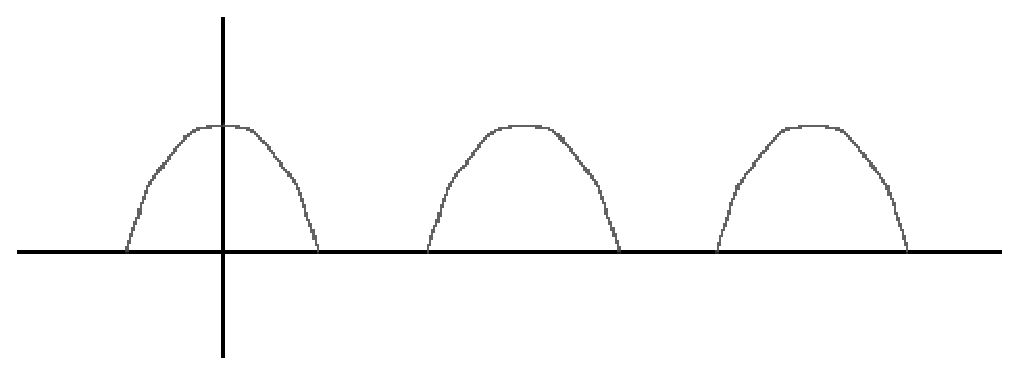
\includegraphics[width=0.8\linewidth,keepaspectratio]{fig/fig2_4.eps}
\caption{標本値のFourier変換。y軸のあたりに現れる原信号が、右側に等間隔で再度現れている}\label{fig2_4}
\end{figure}

このとき、同一のスペクトルの「ズレ」は$\frac{2\pi}{T}$という周波数になり、原信号のスペクトルの両裾とスペクトルの中心(0)間の距離は原信号の最大周波数に相当する。この裾同士が重なり合わないようにサンプリングできれば、1つの山=原信号だけを取り出すことができる。したがって、「ズレ」の間に原信号のスペクトル1つ分がすっぽり入れば良い。式でいうところでは、$\frac{2\pi}{T}$の間に原信号のスペクトル1つ分=最大周波数の2倍が入れば良いということになるので$\frac{2\pi}{T}$は最大周波数の2倍より大きければいいということになる。ここで、$\frac{2\pi}{T}$はサンプリング周期の逆数と$2\pi$をかけたものであるから、サンプリング周波数そのものである。

\section{標本値の量子化}
標本値を取得することで、アナログデータから離散値=デジタルデータを抜き出すことが出来た。しかし、これではまだ記録するには不十分である。というのは、標本値は必ずしも表現可能な数値とは限らないためである。

端的な例として、1辺が1の正方形の対角線の長さを考えよう。三平方の定理を鑑みればその長さが$\sqrt{2}$であることは明らかである。しかし、我々はこれを数値としてそのまま完全に保持することは出来ない。なんとならば、$\sqrt{2}$は無限に続く上に分数としても表現できない、無理数だからである。有限の10進値なり2進値なりで保持あるいは計算するというデジタルデータの原則に沿う限りにおいて、$\sqrt{2}$を保存するには無限の状態が必要となる。無論現実に無限の状態を用意できるわけもないため、必要な精度を以って我々はデータを丸める。つまり、切り捨てたり切り上げたりして表現可能にした近似値を$\sqrt{2}$の値として保存する。

実際には表現可能な数の一覧を尺度として準備しておき、このうち最も近い値として保存する。保存された値のことを量子化値と呼ぶ。量子化のレベル(尺度)は線形軸とする場合が多く、その幅こそ異なれど表現可能な数値の個数は変わらない。勿論、尺度を細かくするほど必要なデータも大きくなる。同じデータであっても線形$256$段階に分けるなら$8$ビットが必要となるが、これが線形$64$段階でいいなら$6$ビットで問題ない。この尺度はデータによって必要な精度等によって変わる。$n$ビットに量子化する場合、そのレベル値は$2^n$個になる。例えば、標本化の折に例を挙げたCD-DA規格は16bit=256レベルで、0dbから96dbまでの振幅を対象に量子化している。

まとめれば、量子化というのは、規格等によって用意された$2^n$個の尺度のうち最も近い値に標本値を丸める行為をいう。

\subsection{量子化雑音}
ここまで読んで明らかな通り標本値と量子化値には誤差が生じる。この誤差を\textbf{量子化雑音}\index{りょうしかざつおん@量子化雑音}と呼ぶ。アナログデータをデジタルデータに変換する際に量子化雑音は避けては通れない問題である。

量子化雑音がどれぐらいになるか見てみよう。最大値$H$、最小値$L$のデータを$n$ビットで量子化した場合、その各データの幅$D$は
\begin{equation}
D=\frac{|H-L|}{2^n-1}
\end{equation}
で与えられる(レベル値=目盛りが全部で$2^n$個あるため、その間を等分したもの)。今、最小値を基準にデータを表すとすれば、量子化値$Q$は
\begin{equation}
Q=L+Dk \ (k=0,1,\cdots,2^n-1)
\end{equation}
と記述できる。したがって標本値$S$との誤差は
\begin{equation}
|S-Q|=|S-(L+Dk)|
\end{equation}
となる。勿論、$k$は誤差が最小になるように選ばれる=標本値に近い側に丸められるのが普通であるので、これを仮定すると
\begin{equation}
|S-Q|=|S-(L+Dk)|\le \frac{D}{2}
\end{equation}
であることがわかる。

量子化雑音を小さくする、つまり標本値の再現精度を上げるためには当然ビット数を増やすことになる。しかし、量子化レベルを1bit増やすということは、全ての標本値を表すのに、各々1bitずつ増やして表現することとなるため、無闇に精度をあげるとデータが肥大化してしまう。このため、データの特性に応じて必要限度のbitを確保するのが一般的である。

\section{量子化値の符号化}
先の標本化・量子化を経てアナログデータをデジタルデータに変換できた。この後の保存は勿論先に学んだデジタルデータと同じように符号化して保存することとなる。

このとき、量子化値の性質によっては用いる符号を考慮して圧縮するなどの場合もある。ランレングスにより圧縮を書ける場合もあれば、連続である以上似たような値が続くと考えられることから差分を抽出し、これにエントロピー符号を適用するなどの手法が考えられる。

\section{値の復元}

逆に、符号化されたデータから原データを復元することを考える。基本的には、ここまでの手順を逆行するだけである。

最初に符号を読み取り、量子化値に戻す。これは実質的に(正しい手順で)符号を読むだけである。次に、量子化値を標本値として周波数スペクトルを求め(勿論、量子化値と標本値は別のものである。だが、量子化の手順で見たとおり、量子化値と標本値の差異は量子化雑音として捨てられたものであり、元の標本値をそのまま求めることは出来ない。そのため、量子化値=標本値の近似値を元の近似値として扱うのである。)、標本値以外の箇所における原データの値を計算する。その値を必要な形式で出力すれば、原データが復元できたと言えよう。

\section*{演習問題}
\begin{problems}
\item 光・音・運動の3データ以外の何らかのデータについて、デジタルへの変換なしに記録あるいは保存する方法を例示せよ。% 時計、熱電対、温度計等

\item 文中に出てきたCD-DAにおいては、44.1kHzのサンプリング周波数で16bit量子化している。また、ステレオ再生とするため、原データは2つに分かれており、その各々が先の通りサンプリングされている。
\begin{enumerate}
\item 1秒あたり何bitの容量が必要となるか(ビットレート)計算せよ。
\item 長さの異なるCD-DA音源のWaveファイルを4〜5個用意し、その再生時間(秒)と容量(ビット)のグラフを作成してみよ(圧縮されているWaveファイルもあるので、長さに対してあまりにサイズが小さい場合は除外すること)。また、そのグラフを直線で結んだときの傾き(ビットレート)と切片(Waveファイルのヘッダサイズ)を求めよ。(Waveファイルを作成する手っ取り早い方法として、適当なCDアルバム1枚をWaveファイルで取り込む方法を挙げておく。)
\end{enumerate}

\item 量子化雑音による誤差が最大0.05℃に収まるように、気温のデータをサンプリングしたい。期待されるデータの最高気温が60℃、最低気温が-90℃であるとき、量子化値の表現には何bitが必要となるか。
\end{problems}


\part{電気伝送の方法}

\chapter{電気伝送の方式}
\input{chap03}

\chapter{電気信号の同期}
\input{chap04}

\chapter{ベースバンド伝送}
前章では、電気信号が届いた際に問題となる「同期」について記した。では、実際に情報を電気信号に乗せ、送るにはどういう方法を取ればよいだろうか。本章および次章ではまさしく通信の本丸と言える信号の伝送について説明する。本章では伝送方式を概観し、その基本となる伝送方式のベースバンド伝送方式について解説を行う。

\section{信号伝送方式}

コンピュータに記録されたデータはbitにより構成されている。この構成する0と1を意味するように電圧の高低を二元状態に当ててやれば、電圧が情報を表していると言える。この電圧の変化はパルス\footnote{短時間に急峻な変化をする信号のこと。また、通信等の分野においては矩形的な変化をする波もパルスと呼ぶ。}であり、そのまま電圧変化として送信することもできる。このように、信号を変換した波をそのままに伝送する方式を\textbf{ベースバンド伝送}\index{べーすばんどでんそう@ベースバンド伝送}または\textbf{基底帯域伝送}\index{きていたいいきでんそう@基底帯域伝送|see{ベースバンド伝送}}と呼ぶ。

一方、波をそのまま送るのではなく、他の\textbf{搬送波}\index{はんそうは@搬送波}(\textbf{キャリア}\index{きゃりあ@キャリア|see{搬送波}}とも)に載せて信号を送る手法もある。この手法を\textbf{ブロードバンド伝送}\index{ぶろーどばんどでんそう@ブロードバンド伝送}または\textbf{帯域伝送}\index{たいいきでんそう@帯域伝送|see{ブロードバンド伝送}}と呼ぶ。ベースバンドよりも装置などが複雑になるが、搬送波に載せて信号を送ることによる様々なメリットが必要となることも多いためこちらの方法が取られるものも多い。

本章では、ベースバンド伝送方式の仕組みと利点について見ていく。帯域伝送方式については次章で取り扱う。

\section{ベースバンド伝送方式}
ベースバンド伝送は、古くから有線通信に使われてきており、現代でもLANの通信や固定電話の一部などで利用されている。古くから使われる理由は、単純な方式で実現が容易であるからと言える。

\subsection{ベースバンド伝送方式の要件}
ベースバンド伝送に必要とされる要件は大きく次の3点である。

\begin{itembox}[l]{ベースバンド伝送方式の要件}
\begin{itemize}
\item 連続性の抑圧:0or1が連続するとタイミング抽出がしにくく(=同期が難しく)なるため、連続しすぎないこと。
\item パワースペクトルの集中性:電圧の変化があまり頻繁(高周波)であると、伝送路によって伝えられないことが起こるため、電圧の周波数がある一定の幅に集中しているのが望ましい。
\item 直流平衡:直流遮断特性(機械の保全等のため直流電圧を通さない特性)による遮断の影響が少ないこと。
\end{itemize}
\end{itembox}

これらの要件のため、後に上げるような様々なベースバンド伝送方式が有り、回路や機械の特性に応じて利用方式が変わる。

\subsection{ベースバンド伝送方式の特徴}
ベースバンド伝送は単なる電気の伝送であるため、長距離でなければ比較的単純に装置を準備できる。このように、回路規模が小さいのがベースバンド伝送方式の特徴である。

一方で、一度に一つの信号しか送れない、雑音に弱い、無線通信では実現が難しいなどの難点もある。特に、最初の「1つの信号しか送れない」点は実際の通信において大きな欠点となる。帯域伝送方式を利用することが多いのはこの難点の解消のためであるが、逆に小規模な伝送では不要な(気にしなくてよい)問題であるためにベースバンド伝送も現役で使われていると言える。

\subsection{ベースバンド伝送方式の分類}
ベースバンド伝送方式は、どのような電圧状態を1/0に対応させるかによって分類が分かれる。以下、その各方式について記述していく。尚、通常は電圧0の状態と電圧$E$ないし$-E$の状態を用いることとなるが、以下は便宜のため0と1/-1を使っているとして記述する。

\subsubsection{RZとNRZ}
あるbitを表す単位時間の電圧のうち半分を電圧0に当てる方式を\textbf{RZ方式}\index{RZほうしき@RZ方式}(Return to Zero方式)と呼ぶ。対して特段そのような措置を取らない手法もあり、この場合は\textbf{NRZ方式}\index{NRZほうしき@NRZ方式}(Non Return to Zero方式)と呼ぶ。RZ方式はビットパルスの半分が0となるのでビット同期に都合が良い。	対してNRZ方式は電圧の変化が少なくなるため、電圧の変化が高周波でなくなるという利点がある。
  

\subsubsection{両極方式と単極方式}
先のRZ方式/NRZ方式に加え、電圧変化にどの幅を使うかにより、\textbf{両極方式}\index{りょうきょくほうしき@両極方式}と\textbf{単極方式}\index{たんきょくほうしき@単極方式}の2種類の方式がある。前者は正極(電圧+1)と負極(電圧-1)を各々1/0に割り当てて利用する。後者の単極方式では正極または負極の一方と電圧0の状態を1/0に割り当てる。

図\ref{fig5_1}に、単極・両極のRZ/NRZ方式の例を示す。
\begin{figure}[htbp]
\centering
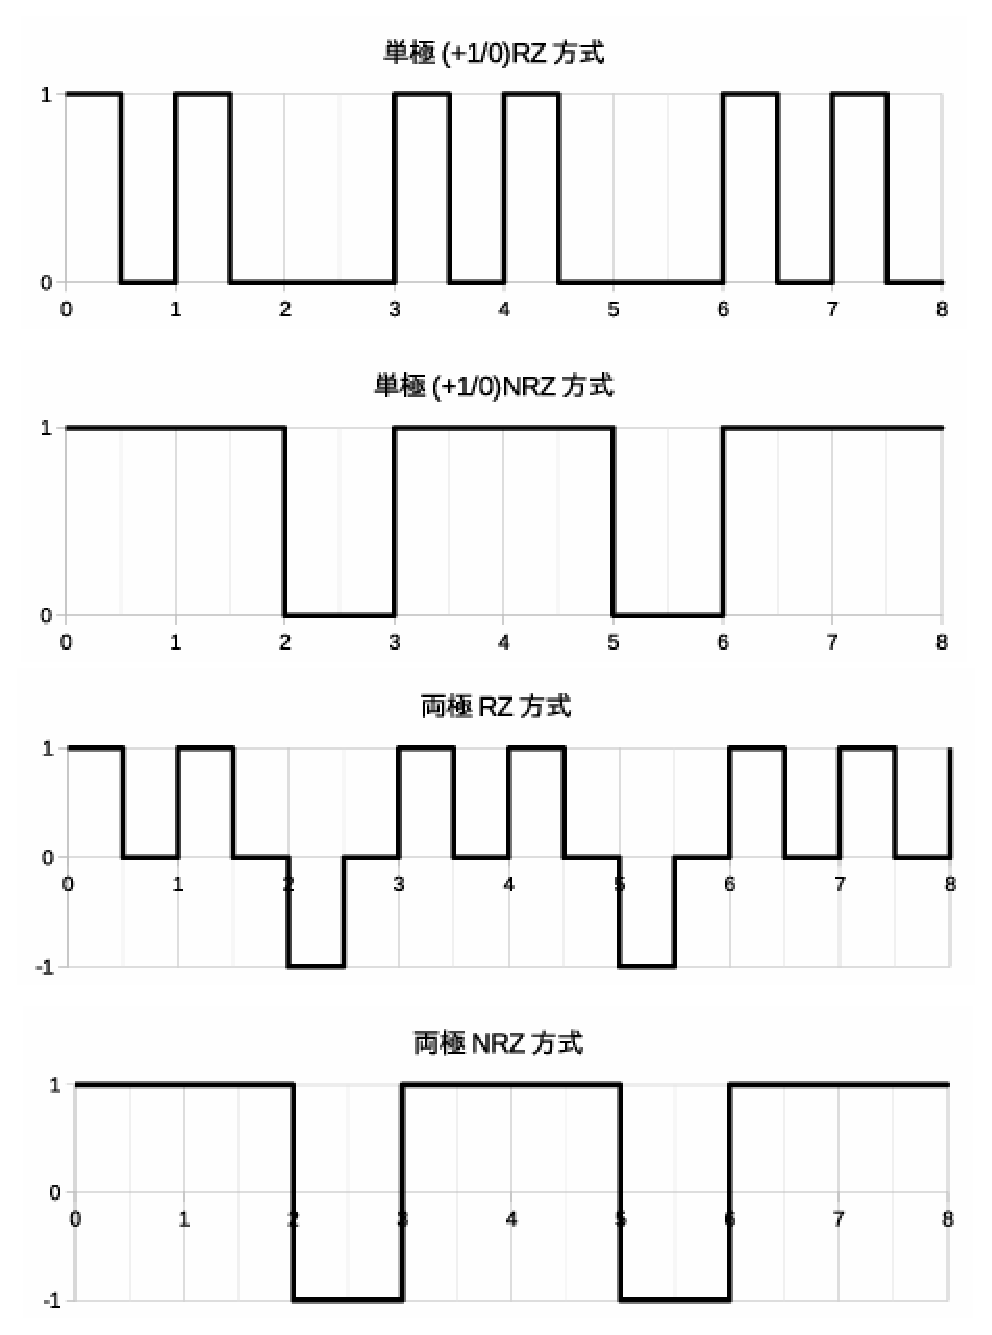
\includegraphics[width=0.8\linewidth,keepaspectratio]{fig/fig5_1.eps}
\caption{単極・両極のRZ・NRZ方式における符号語11011011の電圧変化。横軸の数値はビットの単位時間を示す。}
\label{fig5_1}
\end{figure}

\subsubsection{バイポーラ方式}  
\textbf{バイポーラ方式}\index{ばいぽーらほうしき@バイポーラ方式}(bipolar system)では、正極/負極をともにビット1に当て、電圧0を0に割り当てる。つまり、電圧の絶対値が1/0に対応する。また、1を送り出す場合は「前回1を送ったときと異なる側の極」を使う。つまり、正極を使って1を送った後は(その後にいくつ0があろうとも)次の1は負極を用いて送る。逆もしかりである。この手法では、直流遮断特性の影響を取り除くことができるが、0が連続した場合にビット同期が取り難いという難点もある。

図\ref{fig5_2}に、バイポーラ方式のRZ/NRZ方式の例を示す。
\begin{figure}[htbp]
\centering
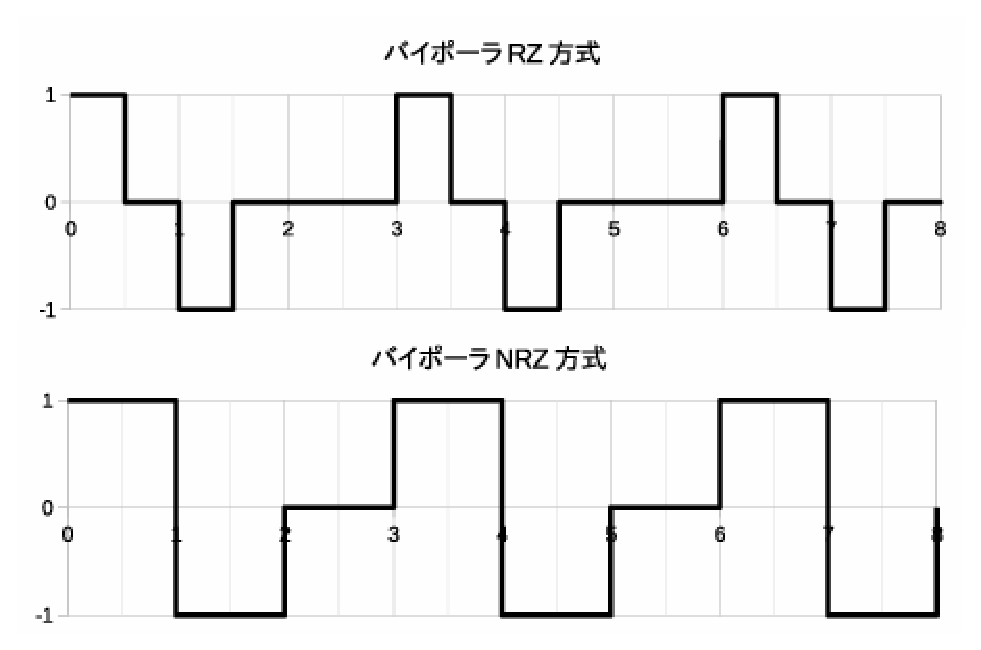
\includegraphics[width=0.8\linewidth,keepaspectratio]{fig/fig5_2.eps}
\caption{バイポーラRZ/NRZ方式における符号語11011011の電圧変化。横軸の数値はビットの単位時間を示す。}
\label{fig5_2}
\end{figure}


\subsubsection{差分方式} 
\textbf{差分方式}\index{さぶんほうしき@差分方式}(differential system) は前の単位時間の電圧から電圧に変化があった場合は1を、なかった場合には0を示す方式である。例えば、ある初期状態の電圧が-1であり、次の単位時間が1、その次の単位時間でも1だったとすると、これは10という符号語になる。

図\ref{fig5_3}に、差分NRZ方式の例を示す(RZ方式では各単位時間後半を0にした図となる)。
\begin{figure}[htbp]
\centering
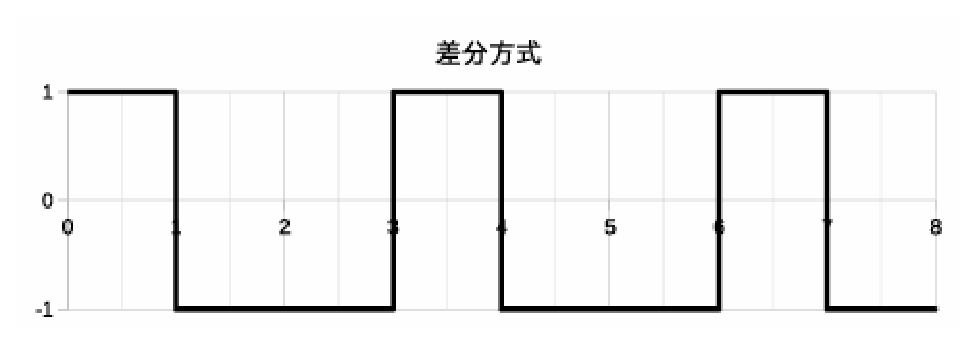
\includegraphics[width=0.8\linewidth,keepaspectratio]{fig/fig5_3.eps}
\caption{差分NRZ方式における符号語11011011の電圧変化。グラフに出ていないが初期状態は-1としている。横軸の数値はビットの単位時間を示す。}
\label{fig5_3}
\end{figure}


\subsubsection{ダイコード方式} 
\textbf{ダイコード方式}\index{だいこーどほうしき@ダイコード方式}(dicode system)では現在のビットが1から0へ変化する場合-1,0から1へ変化する場合1、変化しない場合0の電圧によって表す。初期状態のビットが0であるとして、1の電圧,0の電圧,-1の電圧と続いた場合の符号語は110となる。

図\ref{fig5_4}に、ダイコードNRZ方式の例を示す(RZ方式では各単位時間後半を0にした図となる)。
\begin{figure}[htbp]
\centering
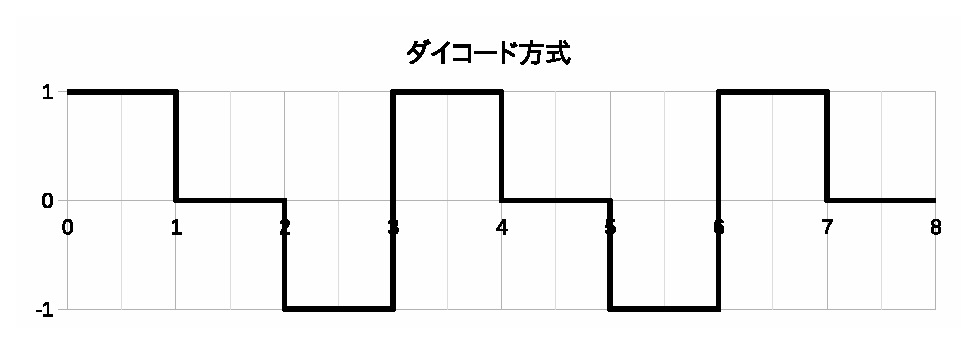
\includegraphics[width=0.8\linewidth,keepaspectratio]{fig/fig5_4.eps}
\caption{ダイコードNRZ方式における符号語11011011の電圧変化。グラフに出ていないが初期状態は0としている。横軸の数値はビットの単位時間を示す。}
\label{fig5_4}
\end{figure}


\subsubsection{マンチェスター/ダイパルス方式}
\textbf{マンチェスター方式}\index{まんちぇすたーほうしき@マンチェスター方式}(Manchester system)あるいは\textbf{ダイパルス方式}\index{だいぱるすほうしき@ダイパルス方式|see{マンチェスター方式}}(dipulse system)は0・1で180度位相の違うパルスを送出するものである。通常、ビットの中心で位相を反転させる(このことから、split-phase符号などとも呼ばれる)。例えば最初-1でスタートしてビットの中心で電圧を1に変えた場合1、その逆に最初1でスタートして後半を-1に変えた場合は0とするのである。位相の反転のおかげでビット同期を取りやすく、後述するEthernet LANで用いられている。

図\ref{fig5_5}に、マンチェスター方式のRZ/NRZ方式の例を示す。
\begin{figure}[htbp]
\centering
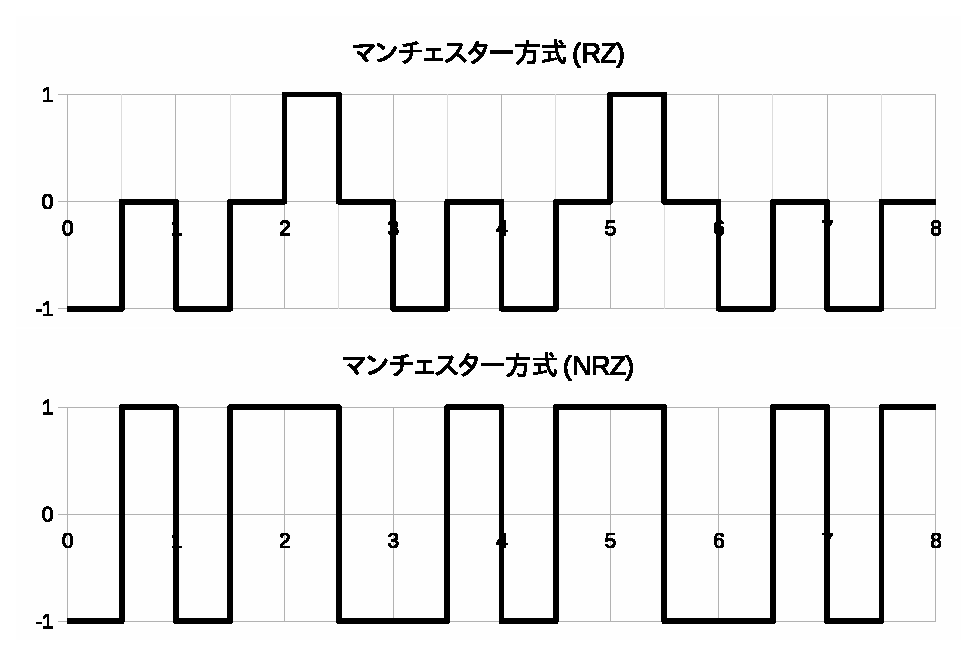
\includegraphics[width=0.8\linewidth,keepaspectratio]{fig/fig5_5.eps}
\caption{マンチェスターRZ/NRZ方式における符号語11011011の電圧変化。横軸の数値はビットの単位時間を示す。}
\label{fig5_5}
\end{figure}
    

\section{伝送速度}
ベースバンド伝送の場合、\textbf{伝送速度}\index{でんそうそくど@伝送速度}は約50kbpsから16Mbpsである。この速度でよく使われる単位"bps"についてここで付章的ながら説明しておく。

bpsはbit/secと書くこともあるが、bit per second(bit毎秒)という単位である。例えば、100bpsは1秒間に100bit=2進数100桁を伝送する速度ということである。似た単位にBpsというのもある。Bを大文字にした場合は一般にByte per second(Byte毎秒)として1秒間に何バイトのデータを伝送するかという単位になる。現在1Byte=8bitであるので、1Bps=8bpsである。

回線速度測定サービスというのがしばしばあるが、これは大きなファイルを用意して、これを送信するのにかかった時間により速度を計算している。300MBのファイルを5分でダウンロードできたとすれば、下りの実効速度\footnote{標榜されている速度ではなく、実際の速度のこと。}は1MBps=8Mbpsとなる。

\subsection{【補足】単位の接頭辞}
\begin{center}
\begin{minipage}[]{0.75\linewidth}
\begin{screen}
\begin{center}
本節は前提知識の補足である。\\
既知の読者におかれては飛ばして次節を読まれたい。
\end{center}
\end{screen}
\end{minipage}
\end{center}

bpsあるいはBps(Byteも含む)単位の接頭辞としては、k(キロ),M(メガ),G(ギガ),T(テラ),P(ペタ)あたりが用いられる。kは$10^3$を示し、以下$10^6,10^9,10^{12},10^{15}$となる。

一方、コンピュータ技術を論ずる場合には、2の累乗が都合が良いため、$10^3=1000$を$2^{10}=1024$に置き換えて用いる場合がある。便宜的にk,M,G,T,Pをそのまま用いる場合もあるが、これを明示する場合にはki(キビ),Mi(メビ),Gi(ギビ),Ti(テビ),Pi(ペビ)という単位(各々$2^{10},2^{20},2^{30},2^{40},2^{50}$)を用いる。

時折、外付けHDDをコンピュータに接続した場合、パッケージ記載の値と容量が異なるように見える場合がある。この原因として、先の$10^3$と$2^{10}$の違いが出てくることがある。例えば1TBのHDDは、$10^{12}$で計算した場合と$2^{40}$で計算すると約100GB,10\%もの違いが出る。

\section*{演習問題}
\begin{problems}
\item 本章内で説明しなかった方式に差動マンチェスタ方式がある。これは、次のようにして定まる。
\begin{itemize}
\item ビットの変わり目で電圧を反対側の極にする(+1なら-1、-1なら+1)。
\item ビットの値が0であれば、1ビット極電圧を維持する。
\item ビットの値が1であれば、ビット中間にてその電圧を反対側の極にする。
\end{itemize}
この差動マンチェスタ方式について、符号語11011011を送る場合、電圧変化はどのようになるか図示せよ。

\item 本章内で出てきた全方式(前問の差動マンチェスタ方式を含む)について、符号語10010011を送る場合の電圧変化を図示せよ。

\item 2000年台前半のソフトウェア公開サイトでは、代表的な速度56kbps(モデム), 64kbps(ISDN), 1Mbps(ADSL), 100Mbps(FTTH)について、ダウンロードにかかる時間が表示されていることがしばしばあった。

ダウンロード対象ファイルのサイズが入力されるとき、先の4回線と自身の好きな速度の1回線でのダウンロード時間を出力するプログラムを作成せよ。ファイルのサイズは小数第2位までの数値と接頭辞(G,M,k,Gi,Mi,ki)及びB(バイト)で入力されるものとする(10.25MBなど。)。なお、入力されるファイルサイズは必ず接頭辞がついてあるものとして良い。

\end{problems}


\chapter{ブロードバンド伝送}
前章で記したとおり、信号伝送方式にはベースバンド伝送とブロードバンド伝送がある。ベースバンド伝送は信号そのものに応じて電圧を変化させて送る方式であった。ブロードバンド伝送ではキャリア(搬送波)にデータを乗せて信号を送る。この章ではまず、キャリアにデータを乗せる手法である\textbf{変調}\index{へんちょう@変調}(modulation)と、キャリアに乗っているデータを取り出す\textbf{復調}\index{ふくちょう@復調}(demodulation)について解説する。次いで、キャリアを複数同時に伝送する方法である多重化について記す。

\section{変調}

帯域伝送においては、キャリアを一つ用意しこれを変化させることでデータを乗せる。つまり、標準的な波(データが乗っていないキャリア単体)からの差分となる部分にデータを乗せるわけである。変調とはキャリアの要素(振幅・周波数・位相)のいずれかをデータに応じて変化させることであり、復調とは逆にキャリアとの差分からデータを取得することである。ベースバンド伝送での電圧の変化方式が複数あったのと同様、キャリアのどの要素を変化させるかによって複数の変調方式がある。

\subsubsection{【補足】波の要素}

\begin{center}
\begin{minipage}[]{0.75\linewidth}
\begin{screen}
\begin{center}
本節は前提知識の補足である。\\
既知の読者におかれては飛ばして次節を読まれたい。
\end{center}
\end{screen}
\end{minipage}
\end{center}

先に、キャリアの要素を振幅・周波数・位相と書いたが、波の要素について補足説明しておく。波の式$w(t)$は、三角関数を用いて以下のように記される(ここでは$\sin$を用いたが、$\cos$を用いても同様である)。
\begin{equation}
w(t)=A\sin (2\pi ft+\theta_0)
\end{equation}
この時、$A$を波の振幅(Amplitude)、$f$を周波数(frequency)、$\theta_0$を位相(phase)と呼ぶ。物理的な意味付としては、振幅:波の最大の振れ幅を示す値、周波数:単位時間あたりに何周期の波が入るか、位相:$t=0$における波の振れがどの程度進んでいるか、ということになる。図\ref{fig6_1}にそれぞれを図解する。

\begin{figure}[htbp]
\centering
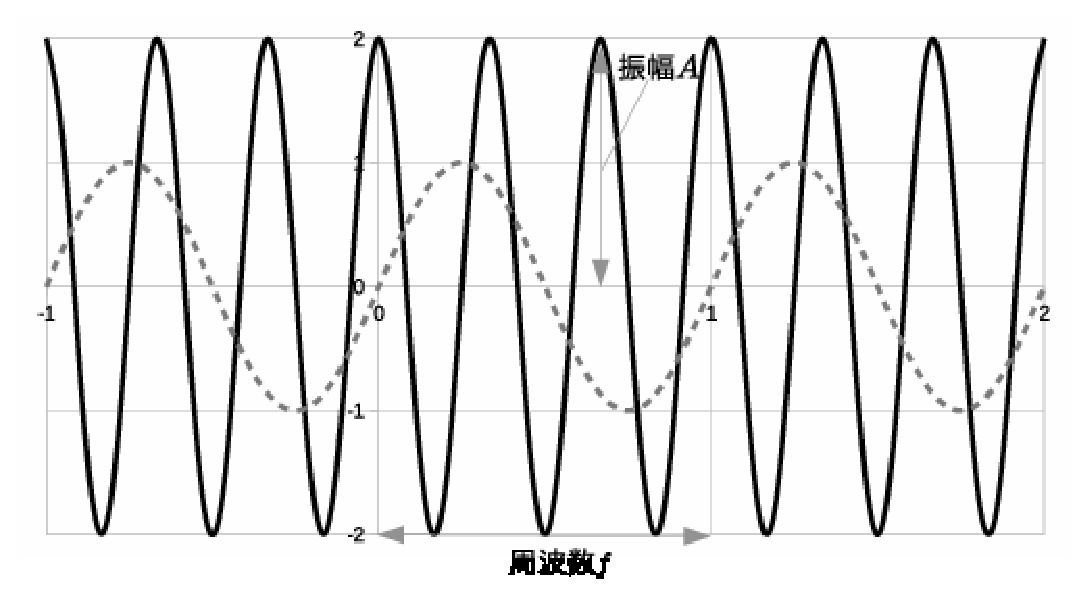
\includegraphics[width=0.9\linewidth,keepaspectratio]{fig/fig6_1.eps}
\caption{波$w_1(t)=\sin 2\pi t$(破線)と波$w_2(t)=2\sin (6\pi t+\frac{\pi}{2})$(実線)の様子。振幅$A=2$と周波数$f=3$を記載。}
\label{fig6_1}
\end{figure}

図\ref{fig6_1}においては、破線により波$w_1(t)=\sin 2\pi t$という位相0、振幅・周波数1という単純な波を示している。また、実線で波$w_2(t)=2\sin (6\pi t+\frac{\pi}{2})$が書かれてあるが、その振れ幅が2倍になっていること、つまり振幅が二ということがわかるであろう。また、周波数についても、0から1の間に、破線の方は1周期の波が入っているのに対し、実線の方は3周期の波が入っている。位相については図の中に書き込めていないが、$w_2(t)$は$t=0$においてちょうど最大振幅まで振れた時、つまり$\frac{\pi}{2}$だけ進んだ時となっている。

このように、振幅・周波数・位相により波の様態は変化する。以降の説明では、これら3要素をどのように変化させるのかを見ていくこととなる。

\subsubsection{【補遺】変調の原理}
\begin{center}
\begin{minipage}[]{0.75\linewidth}
\begin{screen}
\begin{center}
本節は大筋に影響しない。\\
難解あるいは興味索然たるものと感じる折には\\
飛ばして次節を読まれたい。
\end{center}
\end{screen}
\end{minipage}
\end{center}

変調について概念的な説明を行ったが、実現するために数式に落とし込んだ原理を説明しておこう。

出発点はFourier展開の係数の式(\ref{eq_2_2})である。
\begin{equation}
a_k=\int^{L}_{-L} f(x) \cos f_kx dx \quad , \quad b_k=\int^{L}_{-L} f(x) \sin f_kx dx \tag{\ref{eq_2_2}}
\end{equation}

元の信号$f(x)$とキャリア$\cos \omega_c x$の積を取り、このFourier展開を考える。式(\ref{eq_2_2})の$f(x)$を$f(x)\cos \omega_c x$に置き換え、三角関数の積を和に直せば
\begin{equation}
a_k=\frac{1}{2}\int^{L}_{-L} f(x) \left(\cos (\omega_c-f_k) x + \cos (\omega_c+f_k) x \right)dx \label{eq_6_1}
\end{equation}
となる。($b_k$についても、$\cos$を$\sin$に変えた形式で同じである。)キャリアとの積を取った結果、係数における三角関数が上記のように$\pm f_k$だけ変化する。これは、換言すればキャリアの周波数が$\pm f_k$だけ推移したものになる。この推移によってキャリアに信号が乗っているか否か区別でき、またその差異から信号を取り出すことができるのである。

なお、先の推移のうち、正の側を上側波帯、負の側を下側波帯と呼ぶ。信号を取り出すためには一方があれば十分であるため、片方だけを利用するSSB単側波帯通信方式なども実用化されている。

\subsection{振幅変調}

波の3要素のうち、振幅を変えることでデータを乗せる方法を\textbf{振幅変調}\index{しんぷくへんちょう@振幅変調}(Amplitude Modulation,\textbf{AM}\index{AM|see{振幅変調}})と呼ぶ。ラジオにおける中波放送(いわゆるAMラジオ)や短波放送がこの振幅変調により信号を送っている。

送るべき信号の周波数帯に比べて、十分に大きい周波数をもつキャリアを用意する。すると、信号の縮尺でみた時、キャリアはほぼ長方形に塗りつぶしたようなグラフとなる。このキャリアの振幅を信号に応じて変調する(図\ref{fig6_2})。変調後の波は軸の上下両方に信号が乗っていることがわかる。

\begin{figure}[htb]
\centering
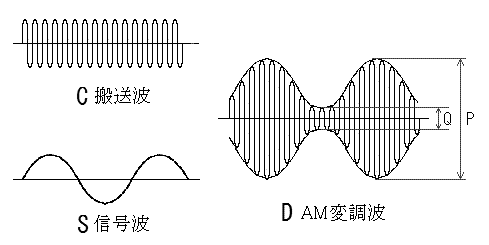
\includegraphics[width=0.6\linewidth,keepaspectratio,bb=0 0 489 245]{fig/fig6_2.png}
\caption{振幅変調のグラフ。Asunaro-net(アスナロネット)より引用}\label{fig6_2}
\end{figure}

同じことを式で示す。伝送する信号(原信号)として正弦波$f(t)=A_s\cos\omega_st$、キャリアとして$f_c(t)=A_c\cos(\omega_ct+\theta_c)$を想定すると(但し、キャリアの仮定から$\omega_s\ll\omega_c$)、振幅変調によりキャリアは振幅項$A_c$が$A_c+f(t)$に置き換わり、全体として次のように表せる。
\begin{eqnarray}
f_c(t)&=&(A_c+A_s\cos\omega_st)\cos(\omega_ct+\theta_c) \nonumber \\
&=&A_c\left(1+\frac{A_s}{A_c}\cos\omega_s t\right)\cos(\omega_ct+\theta_c) \label{eq_6_2}
\end{eqnarray}
ここで$m=A_s/A_c$(図\ref{fig6_2}の$P,Q$を用いると$m=(P-Q)/(P+Q)$とも表せる)は\textbf{変調度}\index{へんちょうど@変調度}(modulation degree)と呼ばれ、変調の深さの程度を表す。変調度の値が大きいほど信号波の振幅が大きくなりクリアになる。ただし100\%を超える状態(過変調)となると、復調信号の波形が歪み、また不要波を発生して他の通信に妨害を与えてしまうので、放送では変調度の最大値が厳しく規定されている。

これによって届いた信号の上半分(半波整流という方法で得られる)の包絡線をとり、直流除去することで復調を実現できる。包絡線を取る手段には、コンデンサの充放電を利用して包絡線を再現する包絡線検波器が一般的である。また、ハイカットフィルター(高周波数成分を除去する)をかけることで包絡線を取ることもできる。

なお、ディジタルデータの伝送ではASK(Amplitude Shift Keying)又はOOK(On Off Keying)とも呼ばれ、0に対しては無変調、1に対しては変調という取扱をすることが多い。伝送路で発生する雑音やレベル変動に弱いものの、非常に安価な回路で実現できること、伝送帯域を有効利用できること、非同期信号の伝送が可能であることといった利点を有する。

\subsubsection{【補遺】振幅変調における周波数推移の例}
\begin{center}
\begin{minipage}[]{0.75\linewidth}
\begin{screen}
\begin{center}
本節は大筋に影響しない。\\
難解あるいは興味索然たるものと感じる折には\\
飛ばして次節を読まれたい。
\end{center}
\end{screen}
\end{minipage}
\end{center}

キャリアの周波数推移が変調の原理であることは既に述べた。ここでは、振幅変調で実際に周波数推移を見てみよう。

式(\ref{eq_6_2})は次のように展開できる。
\begin{eqnarray}
f_c(t)&=&A_c\cos(\omega_ct+\theta_c)+A_cm\cos\omega_st\cdot\cos(\omega_ct+\theta_c) \nonumber \\
&=&A_c\cos(\omega_ct+\theta_c)\nonumber \\
&\ &\quad +\frac{A_cm}{2}\left[\cos\{(\omega_c-\omega_s)t+\theta_c\}+\cos\{(\omega_c+\omega_s)t+\theta_c\}\right] \label{eq_6_3}
\end{eqnarray}

これより振幅変調の結果、周波数領域では$\omega_c$とそれより$\pm\omega_s$だけ離れた成分、$-\omega_c$とそれより$\pm\omega_s$だけ離れた成分が発生していることがわかる。

\subsection{周波数変調}
信号の強度に応じて、キャリアの周波数を変える変調方式を\textbf{周波数変調}\index{しゅうはすうへんちょう@周波数変調}(Frequency Modulation,\textbf{FM}\index{FM|see{周波数変調}})と呼ぶ。デジタル伝送の場合はFSK(Frequency Shift Keying)とも呼ばれる。FNラジオやアマチュア無線などで広く利用される。

送るべき信号の周波数帯に比べて、十分に大きい周波数をもつキャリアを用意する。ここまでは振幅変調と同様である。この時、信号の強度に応じて周波数を変化させる(図\ref{fig6_3})。

\begin{figure}[htb]
\centering
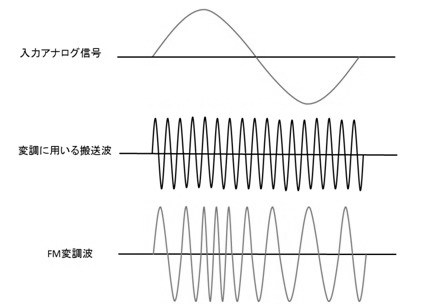
\includegraphics[width=0.6\linewidth,keepaspectratio,bb=0 0 422 307]{fig/fig6_3.jpg}
\caption{周波数変調のグラフ。EDN Japan 「これだけは知っておきたいアナログ用語:FM変調」より引用}\label{fig6_3}
\end{figure}

ただし、そのまま周波数を変更すると復調の際に問題がおこるため、実際には信号の積分を位相に付け加える。伝送する信号(原信号)として正弦波$f(t)=A_s\cos\omega_st$、キャリアとして$f_c(t)=A_c\cos(\omega_ct)$を想定するとき(簡単のため、位相項を省いている)、キャリアの許容する最大の周波数変化を$\delta \omega$として
\begin{equation}
f_c(t) = A_c \cos\left(\omega_c t+\frac{\delta \omega}{\omega_s}\sin\omega_s t\right) \label{eq_6_4}
\end{equation}
とするのが周波数変調である。なお、$m=\delta \omega/\omega_s$が周波数変調における変調度である。これが大きいほど専有帯域が広くなってしまうが、S/N比が向上する。復調の際には、搬送波を微分回路などに通して微分した後、整流・直流カットすることで信号を取り出す。

周波数変調の利点は、振幅が一定であることからノイズに強いということである。振幅方向のノイズは振幅制限器により容易に取り除け、先に書いたように変調度の調整でS/N比の向上も可能である。また、弱肉強食特性と呼ばれる特性があり、弱い信号が混信したとしても先の振幅制限機の都合取り除かれる。これは、混信防止の観点では役に立つが、より強い通信により遮られうるということでもある。

\subsection{位相変調}
\textbf{位相変調}\index{いそうへんちょう@位相変調}(Phase Modulation,\textbf{PM}\index{PM|see{位相変調}})とは、キャリアの位相を変える変調方式であるが、先の周波数変調でも周波数とは言い条、実のところ位相を変更していた。つまり、周波数変調と位相変調は本質的に同じものとなる。しかし、これはアナログの場合の話であり、デジタルデータの伝送、PSK(Phase Shift Keying)の場合にはまた異なる様相を呈する。

デジタル伝送における振幅変調、周波数変調、位相変調(つまりASK,FSK,PSK)の概念を図\ref{fig6_4}に示す。
\begin{figure}[htb]
\centering
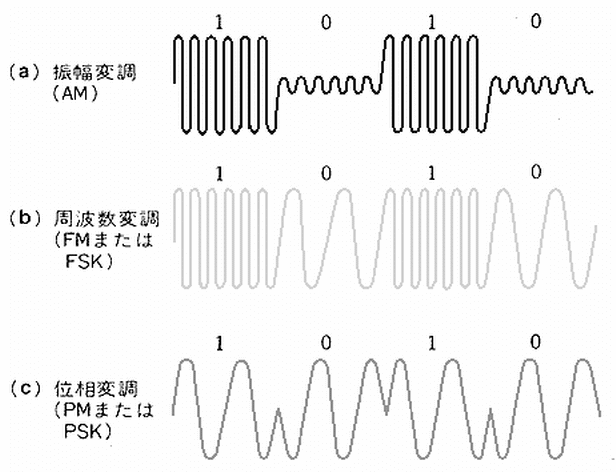
\includegraphics[width=0.6\linewidth,keepaspectratio,bb=0 0 616 472]{fig/fig6_4.png}
\caption{デジタル変調の概念図。宮崎技術研究所サイトより引用}\label{fig6_4}
\end{figure}

ASK,FSKは各々AM,FMを0,1に対応させたということで理解できるであろう。しかし、PSKの場合、FSKとはまるきり異なり、0の波形と1の波形の位相がちょうど180度変わっている。つまり、アナログな伝送においては周波数変調が復調の都合から結果的に位相に頼っている所、デジタル変調ではその事情が変わるゆえに位相変調と周波数変調がはっきりと分かれるのである。

デジタル変調における位相変調には幾つかの手法があるが、ここではBPSKとQPSKを紹介する。

\subsubsection{BPSK}

位相変調の最も基本的なものが、Binary PSK,\textbf{BPSK}\index{BPSK}である。この方式では、ある位相の波とちょうど180度違う波とをそれぞれ0/1に対応させる(図\ref{fig6_5})。これは、二元値となるため雑音に強いという長所がある。特に伝送路の状態に応じて適切な通信速度に変えていくようなプロトコルを用いる場合は、初期のデータリンクを確立させるフェーズでは、このBPSKで通信を開始することが多い。

\begin{figure}[htb]
\centering
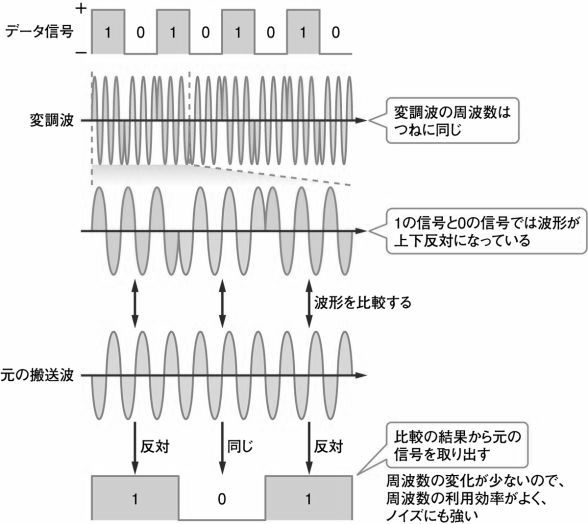
\includegraphics[width=0.8\linewidth,keepaspectratio,bb=0 0 588 524]{fig/fig6_5.jpg}
\caption{BPSKの概念図。ASCII.jp「きっちり知りたい無線LANの変調技術の基礎」より引用}\label{fig6_5}
\end{figure}

\subsubsection{QPSK}

BPSKでは180度違う位相により0と1を表したが、今度は90度ずつ違う4つの位相を用いることにしよう。すると、この結果として4値=00,01,10,11を表すことができる。この手法がQuadrature PSK,\textbf{QPSK}\index{QPSK}である(図\ref{fig6_6})。BPSKと同じ搬送波を用いていても、表すデータ量が2倍に増えているので2倍の伝送速度となる。この手法は、携帯電話の通信で使われる。他、Wi-fi等を定めたIEEE802.11シリーズでは直前の状態との差分データをこの手法により伝送するDQPSK(Differential QPSK)が使われている。

\begin{figure}[htb]
\centering
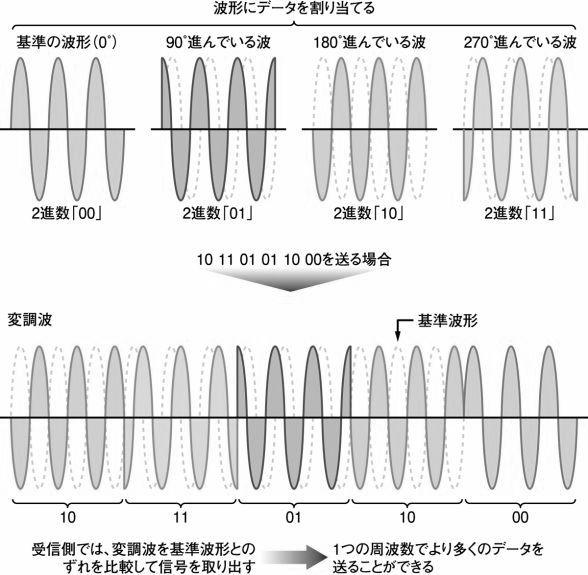
\includegraphics[width=0.8\linewidth,keepaspectratio,bb=0 0 588 575]{fig/fig6_6.jpg}
\caption{QPSKの概念図。ASCII.jp「きっちり知りたい無線LANの変調技術の基礎」より引用}\label{fig6_6}
\end{figure}

しかし、2値を4値にして位相にしたということは、誤差として許容できる位相のズレが半分になったということである。したがって、当然にBPSKよりは雑音に弱くなっている。

これと同じ考えを用いて、8位相を使い3bitを送るものに8PSKがある。更に細かくしていけば16PSKや32PSKなども考えられるが、雑音の影響などから実用的に使われているのは8PSKぐらいまでである。

\subsubsection{変調速度}

デジタル変調では、図\ref{fig6_4}の例からわかるようにキャリアの何周期かに対してデータを対応させて伝送するのが普通である。言い換えれば、キャリアの何周期かを用いて1回の変調を行うということである。キャリアは1秒あたりに$f_c$(周波数)回の周期を持つから、結局1秒あたりに何度の変調を行うかがわかる。このようにして求められる1秒間の変調回数を\textbf{変調速度}\index{へんちょうそくど@変調速度}と呼ぶ。通常、1秒間の変調回数はBaud(ボー)という単位で表す。

昔のモデムなどには、その速度の指標として変調速度が記述されていた。一方、インターネットの普及以後は、伝送速度にはbps(bit per second)が使われる。これらの変換は容易である。1回の変調により何bitのデータとなるのかが分かれば、変調速度に1回あたりのデータ長をかけることでbpsに変換できる。BPSK方式であれば1baud=1bpsであるし、QPSK方式であれば1baud=2bpsである。

\subsection{変調方法の組み合わせ:QAM}
%https://ascii.jp/elem/000/000/458/458953/index-3.html

\subsection{パルス符号変調(PCM)}



\section{多重化}


\section*{演習問題}
\begin{problems}
\item 一般に、AMラジオよりもFMラジオの方がクリアな音声になると言われる。この理由を説明しなさい。

\item ADSLモデムでは、音声通話で利用しない周波数帯域で複数の搬送波を使ってデータ通信を行います。搬送波の数が200であり、各搬送波について1変調あたり128値、変調速度1000ボーであったとすると、伝送速度は何Mbpsになるか求めなさい。
\end{problems}


\chapter{誤り制御}
ここまでに紹介したような方法で十分な水準の通信を確立できる状況となった。しかしながら、どの方法を取るにせよ何らかの事情で通信に誤りが起こることは避けきれない。そこで、通信において正確性を担保するために、誤りを検知して対処するための\textbf{誤り制御}\index{あやまりせぎいぎょ@誤り制御}(error control)の手法がある。今回はこの誤り制御について紹介していく。

\section{誤り制御}

人間が直接声でやり取りをする際に、不明瞭な発音等により意図が正確に伝わらないことは往々にして起こりうる。例えば、数字の1と7はそれぞれ「いち」「しち」と読むわけだが、文脈からどちらかの判断がつかないようなケースでは聞き間違えは致命的となりうる。「1時からの番組の録画予約をお願いします」と伝えたときに、7時から録画されてしまうと見たい番組が見られない。同じように、アルファベットを伝えるシーンでもb,d,pなどは読みが似ているため、メールアドレスを口頭で連絡するなどの必要があるときには、誤りに注意するであろう。

このように、人間同士が声でやり取りする際に誤りが懸念される場合には、予め対処を取るだろう。簡単な例を挙げると
\begin{itemize}
\item わかりやすいように言い換える:「しち」でなく「なな」、「でぃー」でなく「でー」
\item 通話表を使う:いろはの「い」、Bravoの「b」
\item 復唱して確かめる
\item 文脈を付け加えて確認する:「1時からの〇〇という番組?」
\end{itemize}
などは、誤りなく伝えるための手法と言える。そして、これにより誤りが見つかった場合、相手から正しい情報を再度聞き出すなり、明らかに別とわかるなら自分で考えて修正するなりして誤りをなくす。

通信においても、例えば電圧の都合などでビットが不明瞭である\footnote{例えば、CDであればレーザー刻印が十分深くない、電圧がそもそも境界値周辺で振動しているなど。逆に、前者のような刻印をあえて作ってコピーガードとしている例もある。}、雑音が入った、機器の特性など、様々な事情で誤りが起こりうる。これらの対処を行うのが誤り制御である。とりわけ、致命的な過誤を防ぐためにも、誤り制御は重要と言える。とはいえ、誤り制御にあまり大きなリソースを割くのは難しい。先の人間の例であっても、「1時からの番組の録画予約をお願いします」の、1と7以外の場所の誤りを逐一チェックする(「からの」じゃなくて「までの」ではないか、「録画」でなくて「録音」ではないか、「お願いします」ではなく「お願いしません」ではないか…など)ようなことは普通やらない。つまり、誤り制御には次のような性質が求められる。
\begin{itembox}[l]{誤り制御に求められる性質}
\begin{itemize}
\item 誤りを十分に高い確率(100\%とまでは言えなくてもそれに限りなく近い確率)で検知できること。
\item 大幅なリソースを要しないこと。
\item 誤り制御に関する情報自体に誤りが含まれる可能性を考慮すること。また、その誤りが少ない程度に簡潔な情報であること。
\end{itemize}
\end{itembox}

この性質を満たすような手法を用意し、誤りを検出すれば、後はこれを訂正するだけである。人間の例でわかるとおり、訂正方法は「相手に訂正してもらう(再送してもらう)」か「自分で訂正する(訂正できるだけの情報をもらっておく)」のいずれかである。前者のように、誤りを検出するだけして、誤った場合に再送してもらう方法を\textbf{帰還方式}\index{きかんほうしき@帰還方式}(\textbf{ARQ}\index{ARQ|see{ARQ}},Automatic Repeat reQuest)といい、これに使う符号を\textbf{誤り検出符号}\index{あやまりけんしゅつふごう@誤り検出符号}と呼ぶ。一方、後者のように、誤りを検出すると共にその情報から訂正まで行う方式を\textbf{無帰還方式}\index{むきかんほうしき@無帰還方式}(\textbf{FEC}\index{FEC|see{FEC}},Forward Error Control)といい、これに使う符号を\textbf{誤り訂正符号}\index{あやまりていせいふごう@誤り訂正符号}と呼ぶ。

\subsection{誤り制御の簡単な例}

極めて単純な誤り制御の例を3つほどあげてみよう。ファイルをダウンロードする場合を考える。この時、正確なファイルがダウンロードされたかどうかを確認したい。

最も単純な方法として、そのファイルを複数個ダウンロードし、ビット別に比較するという方法が考えられる。十分な数のファイルをダウンロードし、多数決で各ビットを定めていけば(エラー率が十分低い=伝送基準が十分高い前提の下)正しいファイルが出来上がるだろう。しかし、この方法は本来一つで良いはずのファイルを何度もダウンロードしなければならず、例えばOSのisoファイルなどサイズの大きいファイルを対象とした場合にリソースを大幅に食ってしまう。

そこで、ファイル自体に関するデータを確認するという手法がある。例えば、ファイルサイズが本来のサイズとバイト単位で一致するかどうか確認するのである。バイト単位で一致しなければ過剰あるいは不足があり、明らかに正しいデータではないから、再ダウンロードを行う。この手法はやり取りするデータがごく小さいことからリソースが守られるが、同一サイズでビットが変わっているという(起こりえそうな)ケースには無力である。

他には、ファイル・フォーマットを確かめるという手法がある。マニアックな域ならバイナリを見るような人もいるかもしれないが、最も簡単な方法ならそのファイル自体を開ける状態にして開いてみる。ソフトウェアなら動作させればいいし、isoならマウントするなりディスクに焼くなりする。動画や音声なら再生してみれば良い。このとき、正しく開ければおそらく間違ってはいないだろう。この手法は、通信に関するリソースを要求しないが、開く側でのリソースは決して少なくない。また、サーバに搭載するソフトなど、気楽に試せるものばかりでもない。

ここで挙げた例はいずれも誤り制御であるが、それぞれにリソースや検出できる誤りに違いがある。多くの場合、誤り制御はリソースと対処率のトレードオフと言ってよい。このトレードオフの中で、様々な誤り制御手法が生まれてきた。この後は、順次それを紹介していく。
\section{誤り検出符号}
誤り検出符号は誤り訂正符号よりも通常小回りが利く(サイズが小さい・アルゴリズムが速いなど)ものが多いため、現実的な通信もこちらの方式を採用する場合が多い。また、誤り訂正符号と違い、誤っているかどうかがわかれば対処できるため(後述するが、誤り訂正符号は1ビットまでの誤りなら対応できるがそれ以上は対応できないなどの限界がある)、誤りの状況によらない(通信の輻輳等により発生する集中的な誤り(バースト誤り)にも、散発的に発生する単独の誤り(ランダム誤り)にも対応する)という利点もある。

以下、誤り検出符号の何種類かの方式について記す。

\subsection{パリティビット}
データを送る際に、区切りごとの偶奇(パリティ)を定めてビットを付加してデータを送信する方法ならびにその際に付加するビットを\textbf{パリティビット}\index{ぱりてぃびっと@パリティビット}と呼ぶ。これによる誤り検出は\textbf{パリティチェック}\index{ぱりてぃちぇっく@パリティチェック}という。

最もよくあるケースでは、実データ7bit毎にパリティビット1bitを加え、1byte毎のパリティを一定にするようにする。1byte毎のパリティとは、単純にデータ中の1の個数の偶奇である。例えば、1byte毎に偶数になるようなパリティビットを付加する場合、1110001や1110111のように1が偶数個ある実データには0を付加するし、1100100や1111111のように1が奇数個ある実データには1を付加する。受信側は、1byte毎に1の個数を数え、これが奇数である場合は再送を要求する。

もちろん、偶奇が同じ場合には誤りと判断されないので、2bit・4bit等、偶数個のbitに誤りがあった場合には検出できない。また、7bitに1bitをつける場合は元のデータの7分の8のデータとなり、15\%弱のデータ肥大化となる。

\subsubsection{【補遺】パリティチェックの実送信サイズ}
先にデータ肥大化を15\%弱と書いたが、これはデータの再送分などを考慮しておらず、単純に送信すべきデータの量を見た場合である。この補遺では、パリティチェックを行う場合、再送分なども含めて実送信サイズがどれぐらいになるのか(再送要求は十分無視できるサイズとして)考えてみる。

bit毎の誤り率を$p$とし、$n-1$bit毎にパリティビットを付加して$n$bit毎にデータが区切られるものとする。今、検出できる誤りである、奇数個の誤りが起きる確率$P_\mathrm{err}$\footnote{偶数個のエラーが出る場合は検出されないため無視している。}は
\begin{equation}
P_\mathrm{err}=\sum^{n/2}_{i=1} p^{2i-1} (1-p)^{n-2i+1} {}_n\mathrm{C}_{(2i-1)}
\end{equation}
により与えられる。ここで、検出できる誤りの起きる確率とは再送確率であることに注意する。再送が$k$回必要な確率$P_k$は
\begin{equation}
P_k = P_\mathrm{err}^{k} (1-P_\mathrm{err})
\end{equation}
で与えられる。したがって1データ区切り毎の送信回数(=1+送信回数)の期待値$E$は
\begin{equation}
E=\sum^{\infty}_{k=0} (k+1)P_k
\end{equation}
となる。ここで、$P_k$は$P_\mathrm{err}$を公比とする等比数列であり、当然$|P_\mathrm{err}|<1$であるのでこの無限等比級数は収束する。これをもとに計算すると
\begin{equation}
E=\frac{1}{(1-P_\mathrm{err})}
\end{equation}
となる。したがって、再送を平均して$\frac{n}{(1-P_\mathrm{err})}$bitの送信を行うこととなる。元のデータのサイズは区切り毎に$n-1$bitであるから、倍率でいえば$\frac{n}{(n-1)(1-P_\mathrm{err})}$倍のデータサイズとなる。

\subsection{チェックディジット}
符号だけでなく、実データにもよく使われる方法として、\textbf{チェックディジット}\index{ちぇっくでぃじっと@チェックディジット}と呼ばれる方法がある。パスワードやISBNなどにしばしば使われる。

チェックディジットは、データの区切り毎に(通常、そのデータを整数値とみて)何らかの計算を行い、その値を区切り毎に置くという手法である。(適当な計算が1の個数の偶奇であり、それに一致する値を置くという場合はパリティビットそのものになる。)ただし、チェックディジットは通常ビットレベルではなく、もう少し大きな単位で行われることが多い。

チェックディジットは「適当な計算」によりさまざまな種類がある(ゲームのデータ等の場合、独自形式のものも存在する)。ここでは、代表的なものを紹介しておく。
% https://qiita.com/yoshi389111/items/00ca7b3ed9ceac904cde
\subsubsection{DR型・DSR型}
DR(Division Remainder)型のチェックディジットは、数値をある値で割った剰余を付加する方法である。値としては、7や9がよく使われ、7DRや9DRと表記する。また、各々後述の7DSRや9DSRと合わせて、セブンチェックやナインチェックと呼ぶ。

元データが9876543だったとする。このときこれを7で割った余りは5、9で割った余りは6である。したがって、7DRの場合98765435というデータを、9DRの場合98765436というデータを送ることになる(チェックディジットを末尾においた)。

また、余りそのものではなく、割る値に対する基数の補数を付す場合もあり、これをDSR(Divide Subtract Remainder)型と呼ぶ。先の例9876543について、7DSRでチェックディジットを付加すると(7-5=2であるため)98765432となり、9DSRだと98765433となる。

運送会社の伝票番号には7DRが使われている。

\subsubsection{モジュラス・ウェイト型}
モジュラス・ウェイト型は、元の10進整数の各桁に適当な重み(ウェイト)をかけた総和をとり(このときウェイトをかけた時点で2桁以上の数が出た場合に、総和をそのままとる場合は一括方式、桁和を用いる場合分割方式と呼ぶ)、別の値での剰余の補数をとってチェックディジットとする方式である。チェックディジットが2桁になる場合は0にする場合が多い。

具体例として、モジュラス11ウェイト2$\sim$7を用いる、マイナンバーや住民票コード、運転免許証番号で用いられる手法を見てみよう。この方式は、次の手法でチェックディジットを決定する。
\begin{enumerate}
\item 数値の各桁に、下の桁から順に2,3,4,$cdots$,7の係数をかける。(おさまらない場合はまた$2$に戻る。つまり、7桁目には2を、8桁目には3を$\cdots$という風にかける)
\item 各桁の結果の総和を求め、これを11で割った剰余を求める。
\item 求めた剰余を11から引き(=補数を求め)、これをチェックディジットとする。ただし、10以上になる場合はチェックディジットを0とする。
\end{enumerate}

試しに、この方式で123456789のチェックディジットを求めてみよう。各桁の値と重み、その積は次のようになる。
\begin{center}
\begin{tabular}{c|ccccccccc}
桁&1&2&3&4&5&6&7&8&9 \\ 
重み&4&3&2&7&6&5&4&3&2 \\ \hline
桁$\times$重み&4&6&6&28&30&30&28&24&18 \\ 
\end{tabular}
\end{center}
一番下の桁$\times$重みの総和を求めると174となる。これを11で割った剰余は9であるので、チェックディジットは11-9=2となる。このチェックディジットを最終桁につけると1234567899となる。

マイナンバーの場合は11桁の数にこれを適用したものを末尾につけて12桁に、免許証番号の場合は最初の10桁にこれを適用したものをつけて11桁、最後に再発行の回数をつけて12桁としている。


さて、先の例は一括方式であったが、分割方式のものもある。クレジットカードなどで使われるモジュラス10ウェイト2・1分割方式は、次のような手順でチェックディジットを決定する。
\begin{enumerate}
\item 数値の各桁に、下の桁から順に2・1の係数をかける。(おさまらない場合はまた3に戻る。つまり、3桁目には2を、4桁目には1を$\cdots$という風にかける)
\item 掛けた値が2桁になった場合は、その十の位の数と一の位の数を足したものを用いる。(分割)
\item 各桁の結果の総和を求め、これを10で割った剰余を求める。
\item 求めた剰余を10から引き(=補数を求め)、これをチェックディジットとする。ただし、10になる場合はチェックディジットを0とする。
\end{enumerate}

この方式で今度は31415926のチェックディジットを求めてみよう。各桁の値・重み・積と分割結果は次のようになる。
\begin{center}
\begin{tabular}{c|cccccccc}
桁&3&1&4&1&5&9&2&6\\
重み&1&2&1&2&1&2&1&2\\ \hline
桁$\times$重み&3&2&4&2&5&18&2&12\\ \hline
分割&3&2&4&2&5&9&2&3\\
\end{tabular}
\end{center}
総和を求めると30となり、剰余は0である。したがって、補数は10になるが、この場合チェックディジットを0とすることとなっているので、最終的に314159260というデータになる。

ここまで見てきてわかる通り、モジュラスの後の数が剰余をとる数、ウェイトの後の数が下の桁からの重みを示す。ISBN13で用いられているモジュラス10ウェイト3・1方式の場合は、下の桁からの重みが3,1の順となり、総和の剰余ならびに補数の基数となるのは10である。

\subsection{チェックサム}
\textbf{チェックサム}\index{ちぇっくさむ@チェックサム}はファイルダウンロード等の場合に特によく使われる手法で、単純にデータ区切り中の一部の数値の合計を別途作成し、この合計値が一致するか否かで誤り検知を行う方法である。例えば、4バイト毎の最後の1バイトの合計などである。

チェックサムは計算が単純ながら検出率がかなり高いため、しばしば使われる。また、この手法がハッシュ関数等後に示す手法の元となっている場合もある。一方、計算が単純であるゆえの欠点として、比較的簡単に数値を合わせることができるため意図的な改竄などには無力である。

\subsection{CRC(巡回冗長検査)}
\textbf{CRC}\index{CRC}(Cyclic Redundancy Check,\textbf{巡回冗長検査}\index{じゅんかいじょうちょうけんさ@巡回冗長検査|see{CRC}})は多項式による除算の剰余を用いて誤り検出を行う手法である。チェックサム以上に偶発的な誤りについての検出精度が高く、また実装や数学的な分析も比較的容易である一方、チェックサムと同じく意図的な改竄には無力である。

CRCでは、元の情報ビット列を除数を示すビット列(通常、各ビットを立てて多項式と見立てて\textbf{生成多項式}\index{せいせいたこうしき@生成多項式}と呼ぶ)で割り、この剰余をとる。ただし、2進数であることと繰り下がりの計算を無視することから、引き算ではなくXOR \footnote{排他的論理和(exclusive or)。二つの集合の一方のみに属するような部分のこと。bitの場合、同じ値のXORは0、異なる値(1と0)のXORは1となる。bit毎のXORは繰り上がりのない二進加算(=繰り下がりのない二進減算)と同じである。}を行う。とった剰余を元の情報ビット列に付加することで一つの情報となる。

例として、USBの通信に出てくるUSBトークンパケット\footnote{続くパケットがINかOUTかを示すなど、通信制御の役割を持つ。}で用いられているCRC-5-USBを見てみよう。

今、10110001という情報が送られるとする。CRC-5-USBの生成多項式は$x^5+x^2+1$、bit列で表すと100101である。除算の筆算の形式(ただし、商と除数は省略)で書けば、
\begin{center}
\begin{tabular}{c|cccccccc}
元の数&1&0&1&1&0&0&0&1\\
最上位からXOR&1&0&0&1&0&1& & \\ \hline
XOR結果& & &1&0&0&1&0&1\\ 
第3位からXOR& & &1&0&0&1&0&1\\ \hline
剰余& & & & & & & &0\\ 
\end{tabular}
\end{center}
となり、剰余は0である(通常の除算の筆算と異なり、引き算ではなくXORである点に注意すること。)。CRC-5-USBの生成多項式は5次(=6bit)であるので、その剰余は4次(=5bit)である。したがって、この剰余を00000として、元のデータに付すことでCRC-5-USBによる誤り検出符号付きデータが作成される。

\section{誤り訂正符号}
誤り訂正符号は、誤り検出符号に比べると複雑な手法が多く、その分データ量も増えるなどの難点がある。一方で、再送要求が生じないため、再送要求による負荷が大きいと考えられる場合や特定時間しか使えない回線などでは重宝される手法でもある。

ここでは誤り訂正符号の例として、ハミング距離による訂正符号と、ハミング符号を紹介する。

\subsection{ハミング距離による訂正符号}
情報のうちbitが異なれば1,同じであれば0を加算し、これを全bitについて行った総和を\textbf{ハミング距離}\index{はみんぐきょり@ハミング距離}と呼ぶ。$n$ビットの情報$a,b$の$i$ビット目を$a_i,b_i$と記せばハミング距離$H$は
\begin{equation}
H=\sum^{n}_{i=1} \left(1-\delta_{a_ib_i}\right)
\end{equation}
と書ける。ただし、$\delta_{ij}$はクロネッカーデルタ\footnote{$i$と$j$が同じ場合は1、異なる場合は0を返すという関数。}である。

今、3bitの符号のうち、000,111の2つの符号(ハミング距離が3であるような符号)のみを正しい情報とし、それ以外は利用しない符号であるとする。このとき、3bitに対して最大1bitしか誤らないという仮定をおけば、ある3bitが010になるなど、本来あり得ない値が来た場合にハミング距離が短い側の符号にすることで訂正できる。もちろん、2bit以上の誤りの場合は誤った側に解釈してしまうし、3bit使っていながら2値であるので元のデータよりもかなり大きなデータとなってしまうが、先の仮定が成り立つ状況かつ元データのサイズが小さい場合などに確実で容量も一定の伝送ができるともいえる。

同様に、ハミング距離がある一定値の符号の組を用意してそれ以外は使わず、誤ったデータが来た場合近い側に合わせるという手法で比較的単純な訂正符号となる。

\subsection{ハミング符号}
\textbf{ハミング符号}\index{はみんぐふごう@ハミング符号}は、パリティビットをさらに拡張した方式で、元データのうち選択的に選ばれた何ビットかのパリティビットを複数種用意し、これをデータ末尾に付加することによって誤りの検出のみならず例えば1ビットの訂正を可能にする方法ならびにその符号である。

ハミング符号では、最初、元データの1ブロック(データブロック)とパリティビットを次の手順に従って並べる。
\begin{enumerate}
\item 最初、ビット列が空の状態であると考え、この1bit目から埋めていくとする。
\item ビット列を先頭から順に埋める。以下、現在考えている箇所をハミング符号の第$i$番目とあらわす。
  \begin{itemize}
  \item $i$が$2$の累乗数であるとき、このビットはパリティビットとする。
  \item $i$が$2$の累乗数でないとき、データブロックのまだ取っていないビットのうち、先頭のものをハミング符号に含める。
  \end{itemize}
\item 前項をデータブロックが尽きるまで行う。
\end{enumerate}

この手順に従って、例えばbit列の15bit目までを記述すると表\ref{table7_1}($d$は元データのデータブロック、$p$はパリティビットを示し、各々添え字は何番目かを示す)になる。
\begin{table}[htb]
\centering
\caption{ハミング符号のパリティ決定用bit列 15bit目までのビット内訳}\label{table7_1}
\begin{tabular}{|c||c|c|c|c|c|c|c|c|c|c|c|c|c|c|c|}\hline
ビット列の番号&$1$&$2$&$3$&$4$&$5$&$6$&$7$&$8$&$9$&$10$&$11$&$12$&$13$&$14$&$15$\\ \hline
内容&$p_1$&$p_2$&$d_1$&$p_3$&$d_2$&$d_3$&$d_4$&$p_4$&$d_5$&$d_6$&$d_7$&$d_8$&$d_9$&$d_{10}$&$d_{11}$\\ \hline
\end{tabular}
\end{table}

ここで、$i$番目のパリティビット$p_i$は、ビット番号を2進表記したときに$2^{i-1}$の位のビットが立っている箇所のパリティビットの役割を果たす。例えば、$p_2$の場合は、$2$の位のビットが立っている番号ということで、ビット列をベースとして2,3,6,7,10,11,14,15bitでのパリティを指す。このとき、一般にはevenとなるような値がパリティとなる(換言すれば、パリティビット以外の対象ビットの1の個数が奇数なら1、偶数なら0である)。元データで言えば、1,3,4,6,7,10,11bit目のXOR総和が$p_2$となる。この計算によって得られたパリティビットを、先の表\ref{table7_1}に加えた符号全体をハミング符号と呼ぶ。

ハミング符号のある1bitに誤りがあった場合、そのbitの関係する箇所でパリティが合わなくなる。例えば、元データの5bit目(表\ref{table7_1}でわかる通り、ビット列で言うと9番目)に誤りがあった場合、$9_{(10)}=1001_{(2)}$であることから、$p_1$と$p_4$が合わなくなる。1bitの誤りである仮定の下この誤り方は一意に定まるため、何bit目が誤っているか特定・訂正できる。

ハミング符号を付す場合は、パリティビットを$2^m$の単位でつけることから、ブロック長を$2^m-1$とする。この内訳はパリティビットが$m$個、元データが$2^m-1-m$個である。このときのハミング符号をHamming($2^m$,$2^m-1-m$)と記す。例えば、Hamming(7,4)は1ブロック当たり7bit,うちパリティビットが3bitで元データが4bitであるようなハミング符号である。以下、このHamming(7,4)での例を見てみよう。

Hamming(7,4)のパリティビット数は3bitである。表\ref{table7_1}をみてパリティを決定すると
\begin{eqnarray*}
p_1&=&d_1 \oplus d_2 \oplus d_4 \\
p_2&=&d_1 \oplus d_3 \oplus d_4 \\
p_3&=&d_2 \oplus d_3 \oplus d_4 \\
\end{eqnarray*}
である。(ただし、$\oplus$はXOR演算を示す。)例えば元データが1101であった場合、$p_1=1,p_2=0,p_3=0$となり、ハミング符号は1010101となる。

では、これが誤って送られて、例えば1010111と来たとしよう。このとき、先のパリティを計算すると$p_1=1,p_2=1,p_3=1$となり、$p_2,p_3$が異なる。この2つに含まれていて$p_1$に含まれないのは$d_3$であるから、誤っているのは$d_3$と分かり、これを0に訂正することができるのである。

\section*{演習問題}
\begin{problems}
\item Linuxディストリビューションのisoファイルなど、大きなファイルのダウンロードには、md5ファイルという誤り検出用ファイルがしばしば用意されている。これはmd5sumという手法による誤り検出である。この手法について調べ、md5sumのどのような性質がダウンロードの確認に適しているのか説明しなさい。

\item ISBN-10(旧ISBN形式)では、9桁の番号にモジュラス11ウェイト$2\sim 10$方式とも呼ばれるモジュラス・ウェイト型のチェックディジットを付加している。このチェックディジットは次のように計算されている。
\begin{enumerate}[1.]
\item 数値の各桁に、下から2,3,4,$\cdots$,10の重みをかけ、各桁の結果の合計を一括方式で求める。
\item 合計を11で割った剰余を求め、その補数を求める(11からその剰余を引く)。
\item 先に求めた補数が11の場合はチェックディジットは0、10の場合はXとする。それ以外の場合は補数そのものがチェックディジットとなる。チェックディジットを末尾につけて一連の番号とする。
\end{enumerate}
10桁のISBNコードと思われる数字とXからなる列が入力されるとき、これが正しいかどうかを判断するプログラムを作成しなさい。ただし、Xは末尾に限り入力されるものとする。

\item 1バイト毎の後半4ビットを足し合わせるチェックサムを考える。例えば、16進数で$(11 22 33)$というデータであれば、$1+2+3=6$がチェックサムである。今、データ\verb|FE DC BA 98 76 54 32 10|があるとき、これを改ざんして、記した方式のチェックサムで検出できないようなデータを作ってみなさい。また、そのようなデータで、元のデータと一切合致しないようなデータも一例作りなさい。

\item 生成多項式$x+1$(除数11)によるCRCはパリティビットであることを証明しなさい。

\item CRC-4-ITUは生成多項式$x^4+x+1$によるCRCである。このとき、剰余が同じとなるような、同じ長さの別情報を2つ見つけなさい。これが似た情報であるほど誤りやすいといえるが、2つの情報は何ビット異なるか?

\item 4bitでハミング距離が3となるような符号の組を一例あげなさい。この符号ではデータ量がどう増え、またどのような誤りなら訂正できるか?

\item 元データファイル及び加えるパリティビットの数$m$が与えられるとき、元データファイルをHamming($2^m$,$2^m-1-m$)でハミング符号化(Encode)するプログラム(Encoder)ならびに、エンコードデータが与えられるときに、元データを訂正して取り出す(Decode)プログラム(Decoder)を作成しなさい。なお、エンコード時に最終ブロックについてbitの数に端数が出た場合、これには0を付してビット長をそろえなさい。また、Encodeファイルのヘッダとして、最初の1byteをパリティビット数、次の1byteを最終ブロックの元データのビット長(端数のビット数)を付すこととし、デコード用の情報としなさい。

\item (発展問題)bit毎の誤り率を$p$とし、$n-1$bit毎にパリティビットを付加して$n$bit毎にデータが区切られ、このセット$N$個によって送信できる一連のデータがあったとする。このとき、このデータにパリティチェックで検出できない誤りが含まれる確率を$p,n,N$を用いて求めなさい。
\end{problems}


\part{コンピュータ・ネットワークの基礎}

\chapter{通信プロトコル}

\chapter{ネットワークの構成}

\chapter{ネットワークアーキテクチャ}

\chapter{ネットワーク機器}

\chapter{Layer1:物理層}

\chapter{Layer2:データリンク層}

\chapter{Layer3:ネットワーク層 (1)IPとアドレス}

\chapter{Layer3:ネットワーク層 (2)ルーティング}

\chapter{Layer4:トランスポート層}

\chapter{Layer5〜7:上位3層}


\part{ネットワーク・プロトコル}

\chapter{ネットワークモデル・再論}

\chapter{telnet}

\chapter{DNS}

\chapter{DHCP}

\chapter{FTP}

\chapter{HTTP}

\chapter{メールに纏わるプロトコル} %SMTP,POP3,IMAP

\chapter{認証に纏わるプロトコル} %Kerberos,LDAP


\part{安定通信網の構築と運用}

\chapter{冗長化}

\chapter{セキュリティ}

\chapter{トラブルシューティング手法の基礎}


\beginappendix
\chapter{解答例・解説}
\input{AppendixA}

%\chapter{一部解説の付記}
%\input{AppendixB}

%\chapter{Cに関連したWebサービス}
%\input{AppendixC}

%\chapter*{参考書籍等紹介}
%\input{book}

%\chapter*{おわりに}
%\input{last}

\printindex

\end{document}
